% Author: Alfredo Sánchez Alberca (asalber@ceu.es)
% !TEX program = xelatex
%----------------------------------------------------------------------------------------
%    DOCUMENT CLASS
%----------------------------------------------------------------------------------------

\documentclass[11pt,a4paper,openright]{book}
  %----------------------------------------------------------------------------------------
  %	PACKAGES AND OTHER DOCUMENT CONFIGURATIONS
  %----------------------------------------------------------------------------------------
  
  % Language settings
  \usepackage{polyglossia}
  \setdefaultlanguage{spanish}
  
  % Margins and layout
  \usepackage[top=3cm, bottom=3cm, left=2.54cm, right=2.54cm]{geometry}
  
  % Math support
\usepackage{amsmath, amssymb}
 % \usepackage{mathspec}

  % Font settings
  \usepackage{unicode-math}
  \setmainfont[Ligatures=TeX]{TeX Gyre Pagella}
  \setmathfont{TG Pagella Math}
  % \setmathfont[math-style=ISO, bold-style=ISO]{texgyrepagella-math.otf}
  
  % Color
  \usepackage{xcolor} % Required for specifying colors by name
  \definecolor{color1}{RGB}{5,161,230}
  \definecolor{color2}{RGB}{238,50,36}
  \definecolor{ocre}{RGB}{243,102,25} % Define the orange color used for highlighting throughout the book
  \definecolor{blueceu}{RGB}{5,161,230} % Blue color of CEU logo
  \definecolor{greenceu}{RGB}{185,209,16} % Green color of CEU logo
  \definecolor{redceu}{RGB}{238,50,36} % Red color of CEU logo
  \definecolor{grayceu}{RGB}{111,107,83} % Gray color of CEU logo
  \definecolor{coral}{rgb}{1,0.5,0.31} % Orange color for graphics
  \definecolor{royalblue1}{rgb}{0.28,0.46,1} % Blue color for graphics
  \definecolor{mygreen}{rgb}{0,0.8,0} % Green color for graphics
  \definecolor{chaptergrey}{RGB}{5,161,230} % Blue color of CEU logo

  % Line breaking
  \usepackage{microtype} 
  \setlength{\emergencystretch}{2em}
  
  % Graphics
  \usepackage{graphicx}
  \usepackage{tikz} 
  \usepackage{eso-pic} % Required for specifying an image background in the title page
  
  % Arrays and tables
  \usepackage{array}
  \usepackage{multirow}
  \usepackage{colortbl}
  \usepackage{booktabs}
  \newcommand{\tcrule}{\arrayrulecolor{color1!50!white}\toprule}
  \newcommand{\mcrule}{\arrayrulecolor{color1!50!white}\midrule}
  \newcommand{\bcrule}{\arrayrulecolor{color1!50!white}\bottomrule}
  
  % Captions
  \usepackage[margin=20pt, font=small, labelfont=bf, labelsep=endash]{caption}
  
  % Floating figures
  \usepackage{subfigure}
  
  % Lists
  \usepackage[shortlabels]{enumitem} % Customize lists
  %\setlist{nolistsep} % Reduce spacing between bullet points and numbered lists
  \setlist[description]{style=sameline,leftmargin=0cm}

  % Columns
  \usepackage{multicol}
  
  % \makeatletter
  % \let\savees@listquot\es@listquot
  % \def\es@listquot{\protect\savees@listquot}
  % \makeatletter

  % hyperlinks
  \usepackage{hyperref}
  \hypersetup{
  pdfauthor = {Alfredo S\'anchez Alberca},
  pdftitle = {Prácticas de Cálculo con Geogebra},
  pdfsubject = {Cálculo},
  pdfkeywords = {Matemáticas, Cálculo, Geogebra},
  pdfcreator = {XeLaTeX with hyperref package},
  pdfproducer = {pdfLaTeX},
  colorlinks = true,
  linkcolor = red,          % color of internal links
  citecolor = green,        % color of links to bibliography
  filecolor = magenta,      % color of file links
  urlcolor = magenta,          % color of external links
  }
  %\usepackage{breakurl}
  
  % Indentation
  %\setlength\parindent{0pt}
  
  % Control of widow orphan lines
  \clubpenalty=10000
  \widowpenalty=10000 
  
  %Code listing formatting
  \usepackage{listings}
  \lstdefinelanguage{morejava}{morekeywords={String}}
  \definecolor{vollgrau}{rgb}{0.9,0.9,0.9}
  \definecolor{colKeys}{rgb}{0,0,1}
  \definecolor{colIdentifier}{rgb}{0,0,0}
  \definecolor{colComments}{rgb}{1,0.5,0}
  \definecolor{colString}{rgb}{0,0.5,0}
  \definecolor{colbackground}{rgb}{0.9,0.9,1}
  \lstset{%
       language=R,
       float=hbp,%
       basicstyle=\ttfamily,%
       identifierstyle=\color{colIdentifier},%
       keywordstyle=\color{colKeys},%
       stringstyle=\color{colString},%
       commentstyle=\color{colCommentsxelatex},%
  %    columns=flexible,%xelatex
  %    columns=fullflexible,%xelatex
       columns=fixed, %xelatex
       tabsize=1,%xelatex
       extendedchars=true,%xelatex
       showspaces=false,%xelatex
       showstringspaces=false,%xelatex
       breaklines=true,%xelatex
       breakindent=10pt,%xelatex
       backgroundcolor=\color{colbackgxelatexround},%
       breakautoindent=true,%xelatex
       captionpos=t,%
       xleftmargin=1em,%
  %    xrightmargin=.5\fboxsep,%
       numbersep=1em,%
       escapechar=\#\RequirePackage[\eu@zf@math]{fontspec}[2008/08/09]
  }
  
  % Set short or lon\RequirePackage[\eu@zf@math]{fontspec}[2008/08/09]ersion desired
  % \usepackage[cort\RequirePackage[\eu@zf@math]{fontspec}[2008/08/09]
  
  %----------------------------------------------------------------------------------------
%	SECTIONS AND SUBSECTIONS
%----------------------------------------------------------------------------------------
%\titleformat*{\section}{\Huge}
%\titleformat*{\subsection}{\Large}


% Chapter and section formatting 
\usepackage[rigidchapters,explicit]{titlesec}
\setlength{\fboxsep}{5pt}
\newlength{\titulolength}
\setlength{\titulolength}{\textwidth} 
\addtolength{\titulolength}{-2\fboxsep}
\addtolength{\titulolength}{-2\fboxrule}
\titleformat{\chapter}[display]
{\bfseries\sffamily}
{\filleft \mdseries \LARGE \color{blueceu} Práctica \Huge\thechapter}
{0.5ex}
{\colorbox{blueceu}{\parbox[t]{\titulolength}{\rule{0mm}{10mm}\Huge\sffamily\filleft\textcolor{white}{#1}}}}
\titleformat{\section}{\normalfont\Large\bfseries\color{blueceu}}{\arabic{section}}{1em}{#1}
\titleformat{\subsection}{\normalfont\large\bfseries\color{blueceu}}{\arabic{section}.\arabic{subsection}}{1em}{#1}
\titleformat{\subsubsection}{\normalfont\normalsize\bfseries\color{blueceu}}{\arabic{section}.\arabic{subsection}.\arabic{subsubsection}}{0.5em}{#1}
\titlespacing{\chapter}{0pt}{0pt}{30ex}
\titlespacing{\section}{0pt}{8ex}{4ex}

%----------------------------------------------------------------------------------------
%	MAIN TABLE OF CONTENTS
%----------------------------------------------------------------------------------------

% \usepackage{titletoc} % Required for manipulating the table of contents
% 
% \contentsmargin{0cm} % Removes the default margin
% % Chapter text styling
% \titlecontents{chapter}[1.25cm] % Indentation
% {\addvspace{15pt}\large\bfseries} % Spacing and font options for chapters
% {\color{gray}\contentslabel[\Large\thecontentslabel.]{1.25cm}} % Chapter number
% {}  
% {\color{gray}\bfseries\hfill\thecontentspage} % Page number
% % Section text styling
% \titlecontents{section}[1.25cm] % Indentation
% {\addvspace{5pt}\bfseries} % Spacing and font options for sections
% {\contentslabel[\thecontentslabel]{1.25cm}} % Section number
% {}
% {\hfill\color{black}\thecontentspage} % Page number
% []
% % Subsection text styling
% \titlecontents{subsection}[1.25cm] % Indentation
% {\addvspace{1pt}\small} % Spacing and font options for subsections
% {\contentslabel[\thecontentslabel]{1.25cm}} % Subsection number
% {}
% {\;\titlerule*[.5pc]{.}\;\thecontentspage} % Page number
% [] 

%----------------------------------------------------------------------------------------
%	MINI TABLE OF CONTENTS IN CHAPTER HEADS
%----------------------------------------------------------------------------------------

% % Section text styling
% \titlecontents{lsection}[0em] % Indendating
% {\footnotesize\sffamily} % Font settings
% {}
% {}
% {}
% 
% % Subsection text styling
% \titlecontents{lsubsection}[.5em] % Indentation
% {\normalfont\footnotesize\sffamily} % Font settings
% {}
% {}
% {}
 
%----------------------------------------------------------------------------------------
%	PAGE HEADERS
%----------------------------------------------------------------------------------------

% Headings and footers
\usepackage{fancyhdr}
\pagestyle{fancy}
\fancyhead{}
\renewcommand{\chaptermark}[1]{\markboth{\thechapter.\ #1}{}}
\fancyhead[LE]{\scshape Matemática Aplicada con Geogebra}
\fancyhead[RO]{\sffamily\slshape \leftmark}
\renewcommand{\headrulewidth}{0pt}
\renewcommand{\floatpagefraction}{.8}
\renewcommand{\textfraction}{.1}


% \usepackage{fancyhdr} % Required for header and footer configuration
% 
% \pagestyle{fancy}
% \renewcommand{\chaptermark}[1]{\markboth{\color{grayceu}\sffamily\normalsize\textit{#1}}{}} % Chapter text font
% % settings
% %\renewcommand{\sectionmark}[1]{\markright{\color{grayceu}\sffamily\normalsize\textit{\thesection\hspace{5pt}#1}}{}} %
% % Section text font settings
% \fancyhf{} \fancyfoot[LE,RO]{\normalsize\thepage} % Font setting for the page number in the footer
% \fancyhead[RE]{{\color{grayceu}\sffamily\normalsize\textit{Pr�cticas de Bioestad�stica con R and RKTeaching}}} % Print the nearest
% % section name on the left side of odd pages
% \fancyhead[LO]{\leftmark} % Print the current chapter name on the right side of even pages
% \renewcommand{\headrulewidth}{0pt} % Removes the rule in the header
% \addtolength{\headheight}{2.5pt} % Increase the spacing around the header slightly
% \renewcommand{\footrulewidth}{0pt} % Removes the rule in the footer
% \fancypagestyle{plain}{\fancyhead{}\renewcommand{\headrulewidth}{0pt}} % Style for when a plain pagestyle is specified
% 
% % Removes the header from odd empty pages at the end of chapters
% \makeatletter
% \renewcommand{\cleardoublepage}{
% \clearpage\ifodd\c@page\else
% \hbox{}
% \vspace*{\fill}
% \thispagestyle{empty}
% \newpage
% \fi}


%----------------------------------------------------------------------------------------
%	THEOREM STYLES
%----------------------------------------------------------------------------------------

\usepackage{amsthm} % For including math equations, theorems, symbols, etc

\newcommand{\intoo}[2]{\mathopen{]}#1\,;#2\mathclose{[}}
\newcommand{\ud}{\mathop{\mathrm{{}d}}\mathopen{}}
\newcommand{\intff}[2]{\mathopen{[}#1\,;#2\mathclose{]}}
\newtheorem{notation}{Notación}[chapter]

\newtheoremstyle{blueceu} % Theorem style name
{7pt} % Space above
{7pt} % Space below
{\normalfont} % Body font
{} % Indent amount
{\small\bf\sffamily\color{blueceu}} % Theorem head font
{\;\;} % Punctuation after theorem head
{0.25em} % Space after theorem head
{\small\sffamily\color{blueceu}\thmname{#1}\thmnumber{\@ifnotempty{#1}{ }\@upn{#2}} % Theorem text (e.g. Theorem 2.1)
\thmnote{\ {\the\thm@notefont\sffamily\bfseries\color{blueceu}--- #3.}}} % Optional theorem note
\renewcommand{\qedsymbol}{$\blacksquare$} % Optional qed square

\newtheoremstyle{blacknumex} % Theorem style name
{7pt} % Space above
{7pt} % Space below
{\normalfont} % Body font
{} % Indent amount
{\small\bf\sffamily} % Theorem head font
{\;\;} % Punctuation after theorem head
{0.25em} % Space after theorem head
{\small\sffamily{\tiny\ensuremath{\blacksquare}}\ \thmname{#1}\thmnumber{\@ifnotempty{#1}{ }\@upn{#2}} % Theorem text (e.g. Theorem 2.1)
\thmnote{\ {\the\thm@notefont\sffamily\bfseries--- #3.}}} % Optional theorem note

\newtheoremstyle{blacknum} % Theorem style name
{7pt} % Space above
{7pt} % Space below
{\normalfont} % Body font
{} % Indent amount
{\small\bf\sffamily} % Theorem head font
{\;\;} % Punctuation after theorem head
{0.25em} % Space after theorem head
{\small\sffamily\thmname{#1}\thmnumber{\@ifnotempty{#1}{ }\@upn{#2}} % Theorem text (e.g. Theorem 2.1)
\thmnote{\ {\the\thm@notefont\sffamily\bfseries--- #3.}}} % Optional theorem note

\newtheoremstyle{example} % Theorem style name
{7pt} % Space above
{7pt} % Space below
{\normalfont} % Body font
{} % Indent amount
{\small\bf\sffamily} % Theorem head font
{\;\;} % Punctuation after theorem head
{0.25em} % Space after theorem head
{\small\sffamily\thmname{#1} % Theorem text (e.g. Theorem 2.1)
\thmnote{\ {\the\thm@notefont\sffamily\bfseries--- #3.}}} % Optional theorem note

\newtheoremstyle{indication} % Theorem style name
{-5pt} % Space above
{7pt} % Space below
{\normalfont} % Body font
{-28pt} % Indent amount
{\bf} % Theorem head font
{\kern-11.5pt} % Punctuation after theorem head
{20pt} % Space after theorem head
{\begin{tikzpicture}
\draw node [fill=blueceu,opacity=1,inner sep=1pt] {\makebox[17pt][c]{
\includegraphics[scale=0.3]{img/bulb}}}; \end{tikzpicture}} % Theorem text (e.g. Theorem 2.1)

\makeatother

% Defines the theorem text style for each type of theorem to one of the three styles above
\theoremstyle{ocrenum}
\newtheorem{exerciseT}{Exercise}[chapter]
\theoremstyle{blacknumex}
\newtheorem{exampleT}{Example}[chapter]
%\theoremstyle{blacknum}
\theoremstyle{blueceu}
\newtheorem{vocabulary}{Vocabulario}[chapter]
\newtheorem{definitionT}{Definición}[chapter]
\newtheorem{theoremT}{Teorema}[chapter]
\newtheorem{corolary}{Corolario}[chapter]
\theoremstyle{indication}
\newtheorem{indicationT}{Indicación}
%\theoremstyle{example}
%\newtheorem{ejemplo}{Ejemplo}

%----------------------------------------------------------------------------------------
%	DEFINITION OF COLORED BOXES
%----------------------------------------------------------------------------------------

\RequirePackage[framemethod=default]{mdframed} % Required for creating the theorem, definition, exercise and corollary boxes

% Theorem box
\newmdenv[skipabove=7pt,
skipbelow=7pt,
backgroundcolor=black!5,
linecolor=ocre,
innerleftmargin=5pt,
innerrightmargin=5pt,
innertopmargin=5pt,
leftmargin=0cm,
rightmargin=0cm,
innerbottommargin=5pt]{tBox}

% Exercise box	  
\newmdenv[skipabove=7pt,
skipbelow=7pt,
rightline=false,
leftline=true,
topline=false,
bottomline=false,
backgroundcolor=ocre!10,
linecolor=ocre,
innerleftmargin=5pt,
innerrightmargin=5pt,
innertopmargin=5pt,
innerbottommargin=5pt,
leftmargin=0cm,
rightmargin=0cm,
linewidth=4pt]{eBox}	

% Definition box
\newmdenv[skipabove=10pt,
skipbelow=10pt,
rightline=false,
leftline=true,
topline=false,
bottomline=false,
linecolor=ocre,
innerleftmargin=5pt,
innerrightmargin=5pt,
innertopmargin=0pt,
leftmargin=0cm,
rightmargin=0cm,
linewidth=4pt,
innerbottommargin=0pt]{dBox}	

% Corollary box
\newmdenv[skipabove=7pt,
skipbelow=7pt,
rightline=false,
leftline=true,
topline=false,
bottomline=false,
linecolor=gray,
backgroundcolor=black!5,
innerleftmargin=5pt,
innerrightmargin=5pt,
innertopmargin=5pt,
leftmargin=0cm,
rightmargin=0cm,
linewidth=4pt,
innerbottommargin=5pt]{cBox}	

% Indication box
\newmdenv[skipabove=7pt,
skipbelow=7pt,
rightline=false,
leftline=true,
topline=false,
bottomline=false,
linecolor=blueceu,
backgroundcolor=black!5,
innerleftmargin=5pt,
innerrightmargin=5pt,
innertopmargin=5pt,
leftmargin=0pt,
rightmargin=0pt,
linewidth=4pt,
innerbottommargin=5pt]{iBox}		  
		  			  


% Creates an environment for each type of theorem and assigns it a theorem text style from the "Theorem Styles" section above and a colored box from above
\newenvironment{theorem}{\begin{tBox}\begin{theoremT}}{\end{theoremT}\end{tBox}}
\newenvironment{exercise}{\begin{eBox}\begin{exerciseT}}{\hfill{\color{ocre}\tiny\ensuremath{\blacksquare}}\end{exerciseT}\end{eBox}}				  
\newenvironment{definition}{\begin{dBox}\begin{definitionT}}{\end{definitionT}\end{dBox}}	
\newenvironment{example}{\begin{exampleT}}{\hfill{\tiny\ensuremath{\blacksquare}}\end{exampleT}}		
\newenvironment{corollary}{\begin{cBox}\begin{corollaryT}}{\end{corollaryT}\end{cBox}}	
\newenvironment{indication}{\begin{iBox}\begin{indicationT} \renewcommand{\theenumii}{\arabic{enumii}}\renewcommand{\labelenumii}{\sffamily\theenumii)}\renewcommand{\theenumiii}{\arabic{enumiii}}\renewcommand{\labelenumiii}{\sffamily\theenumiii)}}{\end{indicationT}\end{iBox}}
%----------------------------------------------------------------------------------------
%	REMARK ENVIRONMENT
%----------------------------------------------------------------------------------------

%\newenvironment{remark}{\par\vskip10pt\small % Vertical white space above the remark and smaller font size
%\begin{list}{}{
%\leftmargin=35pt % Indentation on the left
%\rightmargin=25pt}\item\ignorespaces % Indentation on the right
%\makebox[-2.5pt]{\begin{tikzpicture}[overlay]
%\node[draw=ocre!60,line width=1pt,circle,fill=ocre!25,font=\sffamily\bfseries,inner sep=2pt,outer sep=0pt] at (-15pt,0pt){\textcolor{ocre}{R}};\end{tikzpicture}} % Orange R in a circle
%\advance\baselineskip -1pt}{\end{list}\vskip5pt} % Tighter line spacing and white space after remark

% %----------------------------------------------------------------------------------------
% %	SECTION NUMBERING IN THE MARGIN
% %----------------------------------------------------------------------------------------
% 
% \makeatletter
% %\renewcommand{\@seccntformat}[1]{\llap{\textcolor{grayceu}{\csname the#1\endcsname.}\hspace{1em}}}                    
% \renewcommand{\section}{
% 	\@startsection{section}{1}{\z@}
% 	{-4ex \@plus -1ex \@minus -.4ex}{1ex \@plus.2ex }
% 	{\normalfont\LARGE}
% }
% \renewcommand{\subsection}{
% 	\@startsection{subsection}{2}{\z@}
% 	{-3ex \@plus -0.1ex \@minus -.4ex}{0.5ex \@plus.2ex }
% 	{\normalfont\Large}
% }
% \renewcommand{\subsubsection}{
% 	\@startsection{subsubsection}{3}{\z@}
% 	{-2ex \@plus -0.1ex \@minus -.2ex}{0.2ex \@plus.2ex }
% 	{\normalfont\large}
% }                        
% \renewcommand{\paragraph}{
% 	\@startsection{paragraph}{4}{\z@}
% 	{-2ex \@plus-.2ex \@minus .2ex}{0.1ex}
% 	{\normalfont\bfseries}
% }
% 
% \def\thechapter{\arabic{chapter}}
% \def\thesection{\thechapter.\arabic{section}.}
% \def\thesubsection{\thesection\arabic{subsection}.}
% \def\thesubsubsection{\thesubsection\arabic{section}.}
% 
% %----------------------------------------------------------------------------------------
% %	CHAPTER HEADINGS
% %----------------------------------------------------------------------------------------
% %\newcommand{\thechapterimage}{}
% %\newcommand{\chapterimage}[1]{\renewcommand{\thechapterimage}{#1}}
% \def\@makechapterhead#1{
% \thispagestyle{empty}
% {
% \ifnum \c@secnumdepth >\m@ne
% \if@mainmatter
% \startcontents
% \begin{tikzpicture}[remember picture,overlay]
% % \node at (current page.north west)
% % {\begin{tikzpicture}[remember picture,overlay]
% % 
% % %\node[anchor=north west] at (-4pt,-27.5mm) {\includegraphics[width=\paperwidth]{\thechapterimage}};
% % %Commenting the 3 lines below removes the small contents box in the chapter heading
% % % \draw[fill=white,opacity=.6] (30mm,-30mm) rectangle (9cm,-9cm);
% % % \node[anchor=north west] at (30mm,-30mm) {\parbox[t][9cm][t]{5.5cm}{\huge\bfseries\flushleft \printcontents{l}{1}{\setcounter{tocdepth}{2}}}};
% % % \draw[anchor=west] (5cm,-11cm) node [rounded corners=25pt,fill=white,opacity=.7,inner sep=15.5pt]{\huge\sffamily\bfseries\textcolor{black}{\vphantom{plPQq}\makebox[20cm]{}}};
% \draw[anchor=north west, fill=black] (0mm,50mm) rectangle (1pt,10mm);
% \draw[anchor=north west] (0cm,20mm) node {\scalebox{1.5}{\Huge{\textcolor{grayceu}\thechapter}}}; 
% %\draw[anchor=west] (0cm,0cm) node {\Huge{#1}}; 
% \end{tikzpicture}
% \par\vspace*{2cm}
% {\Huge #1}
% \par\vspace*{1cm}
% % \end{tikzpicture}}\par\vspace*{230\p@}
% }}
% \def\@makeschapterhead#1{
% \thispagestyle{empty}
% {
% \ifnum \c@secnumdepth >\m@ne
% \if@mainmatter
% \startcontents
% \begin{tikzpicture}[remember picture,overlay]
% % \node at (current page.north west)
% % {\begin{tikzpicture}[remember picture,overlay]
% % \node[anchor=north west] at (-4pt,-27.5mm) {\includegraphics[width=\paperwidth]{\thechapterimage}};
% % \draw[anchor=west] (5cm,-11cm) node [rounded corners=25pt,fill=white,opacity=.7,inner sep=15.5pt]{\huge\sffamily\bfseries\textcolor{black}{\vphantom{plPQq}\makebox[20cm]{}}};
% % \draw[anchor=west] (5cm,-11cm) node [rounded corners=25pt,inner sep=15.5pt]{\huge\sffamily\bfseries\textcolor{black}{#1\vphantom{plPQq}\makebox[20cm]{}}};
% % \end{tikzpicture}};
% % \end{tikzpicture}}\par\vspace*{230\p@}
% %\draw[anchor=west] (0cm,0cm) node {\Huge{#1}}; 
% \end{tikzpicture}
% {\Huge #1}
% \par\vspace*{1cm}
% }}
% \makeatother

 % Insert the commands_book.tex file which contains the majority of the structure behind
  % the template
  
  %----------------------------------------------------------------------------------------
  %	COMMANDS FOR INDICATIONS
  %----------------------------------------------------------------------------------------
  \usepackage{menukeys}
  \DeclareFontFamily{\encodingdefault}{\ttdefault}{\hyphenchar\font=`\-}
  \newmenucolortheme{mycolors}{named}{white}{color1}{black}
  \changemenucolortheme{menus}{mycolors}
  \renewmenumacro{\menu}[>]{menus}
  %\newmenustylesimple*{botonstyle}{\textbf{\CurrentMenuElement}}
  %\renewmenumacro{\keys}{botonstyle}
  \newcommand{\button}[1]{\textsf{\small #1}}
  \newcommand{\option}[1]{\textsf{\small #1}}
  \newcommand{\mtab}[1]{\textsf{\small #1}}
  \newcommand{\field}[1]{\textsf{\small #1}}
  \newcommand{\command}[1]{\texttt{#1}}
  \newcommand{\variable}[1]{\textsf{\small #1}}
  \newcommand{\result}[1]{\texttt{#1}}
  
  % OTHERS
  \newcommand{\resetcounters}{\setcounter{page}{1} \setcounter{section}{0} \setcounter{footnote}{0} \setcounter{figure}{0} \setcounter{table}{0}}
  
% MATH OPERATORS IN SPANISH
\newcommand{\sen}{\operatorname{sen}}
\newcommand{\arcsen}{\operatorname{arcsen}}
\newcommand{\tg}{\operatorname{tg}}
\newcommand{\arctg}{\operatorname{arctg}}
\newcommand{\cosec}{\operatorname{cosec}}
\newcommand{\cotg}{\operatorname{cotg}}
\newcommand{\dom}{\operatorname{Dom}}
\newcommand{\im}{\operatorname{Im}}
\newcommand{\dint}{\displaystyle \int}
  
  %========================================================================================
  %   DOCUMENT BODY
  %========================================================================================
\begin{document}
\frontmatter
% Add two blank pages at the begining
%\null\thispagestyle{empty}\newpage
%\null\thispagestyle{empty}\newpage
%----------------------------------------------------------------------------------------
%	TITLE PAGE
%----------------------------------------------------------------------------------------
% \input{preambulo/titulo} 
%\input{preamble/titlepage_book} 

%----------------------------------------------------------------------------------------
%	COPYRIGHT PAGE
%----------------------------------------------------------------------------------------
% % Términos de la licencia Creative Commons 4.0
\thispagestyle{empty}
\null
\vfill
\hrule depth 3pt
\smallskip
\sffamily

\noindent \textbf{Cálculo con Geogebra}\\
Alfredo Sánchez Alberca (asalber@ceu.es) 

\bigskip
% Creative Commons license terms
{\Large \textbf{Términos de la licencia \normalsize \ccLogo}}
\medskip

\small
Esta obra está bajo una licencia Atribución--No comercial--Compartir igual 4.0 Internacional de Creative Commons.
Para ver una copia de esta licencia, visite \url{https://creativecommons.org/licenses/by-nc-sa/4.0/deed.es}.

\medskip
Con esta licencia eres libre de:
\begin{itemize}
\item \textbf{Compatir}: Copiar y redistribuir el material en cualquier medio o formato 
\item \textbf{Adaptar}: Remezclar, transformar y construir a partir del material 
\end{itemize}

Bajo las siguientes términos:
\begin{center}
\begin{tabular}{ccp{10cm}}
\ccAttribution  & \qquad & \textbf{Atribución}. Usted debe dar crédito de manera adecuada, brindar un enlace a la licencia, e indicar si se han realizado cambios. Puede hacerlo en cualquier forma razonable, pero no de forma tal que sugiera que usted o su uso tienen el apoyo de la licenciante.\\
\ccNonCommercialEU & \qquad & \textbf{No comercial}. Usted no puede hacer uso del material con propósitos comerciales.\\
\ccShareAlike & \qquad & \textbf{Compartir igual}. Si remezcla, transforma o crea a partir del material, debe distribuir su contribución bajo la lamisma licencia del original.
\end{tabular}
\end{center}

No hay restricciones adicionales — No puede aplicar términos legales ni medidas tecnológicas que restrinjan legalmente a otras a hacer cualquier uso permitido por la licencia. 

\begin{itemize}
\item Al reutilizar o distribuir la obra, tiene que dejar bien claro los términos de la licencia de esta obra.
\item Alguna de estas condiciones puede no aplicarse si se obtiene el permiso del titular de los derechos de autor
\item Nada en esta licencia menoscaba o restringe los derechos morales del autor.
\end{itemize}

\hrule depth 3pt

\normalfont
\newpage

%----------------------------------------------------------------------------------------
%	TABLE OF CONTENTS
%----------------------------------------------------------------------------------------
%\chapterimage{img/chapter_head.png} % Table of contents heading image
{\pagestyle{plain} % No headers
%\input{registro}
\tableofcontents\thispagestyle{empty}
% Print the table of contents itself
\cleardoublepage % Forces the first cxelatexhapter to start on an odd page so it's on the right
}
\mainmatter
%----------------------------------------------------------------------------------------
%	CHAPTERS
%----------------------------------------------------------------------------------------
% !TEX root = ../practicas_geogebra.tex
% Author: Alfredo Sánchez Alberca (asalber@ceu.es)
\chapter{Introducción a Geogebra}

\section{Introducción}
La gran potencia de cálculo alcanzada por los ordenadores en las últimas décadas ha convertido a los mismos en poderosas herramientas al servicio de todas aquellas disciplinas que, como las matemáticas, requieren cálculos largos y complejos.

Geogebra\footnote{Esta practica está basada en la versión 6.1 de Geogebra Clásico} es uno de los programas de cálculo numérico y simbólico más utilizados.
Aparte de sus capacidades el cálculo numérico, vectorial y matricial, también puede realizar representaciones gráficas, lo cual permite resolver multitud de problemas de Álgebra, Análisis, Cálculo, Geometría e incluso Estadística, de manera interactiva.
La ventaja de Geogebra frente a otros programas habituales de cálculo como Mathematica, Mapple o MATLAB, radica en su sencillez y simplicidad de uso, y en que es software libre, por lo que puede instalarse sin coste alguno e incluso modificarse.

\begin{center}

\includegraphics[scale=0.8]{img/introduccion/geogebra-logo}
\end{center}

El programa puede descargarse de las página web \url{https://www.geogebra.org}.
En esta web existe también una versión en linea del programa que permite usarlo como una aplicación web sin necesidad de instalarlo en el ordenador.
Esta web dispone también de multitud de tutoriales y recursos educativos a disposición de los usuarios.
De hecho, cualquier usuario puede registrarse y subir a esta web actividades desarrolladas con Geogebra.

El objetivo de esta práctica es introducir al alumno en la utilización de este programa, enseñándole a realizar las operaciones básicas más habituales en Cálculo.

\section{Arranque}
Como cualquier otra aplicación de Windows, para arrancar el programa hay que pulsar sobre la opción correspondiente del menú \menu{Inicio>Programas}, o bien sobre el icono de escritorio 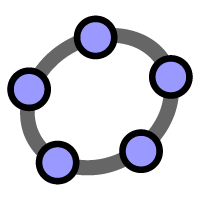
\includegraphics[scale=0.04]{img/introduccion/geogebra-icon}.

Cuando el programa arranca, en la pantalla aparece la ventana de inicio del programa (figura \ref{g:ventana-inicio}), que nos permite seleccionar distintos entornos de trabajo o \emph{Apariencias}.

\begin{figure}[h!]
\begin{center}
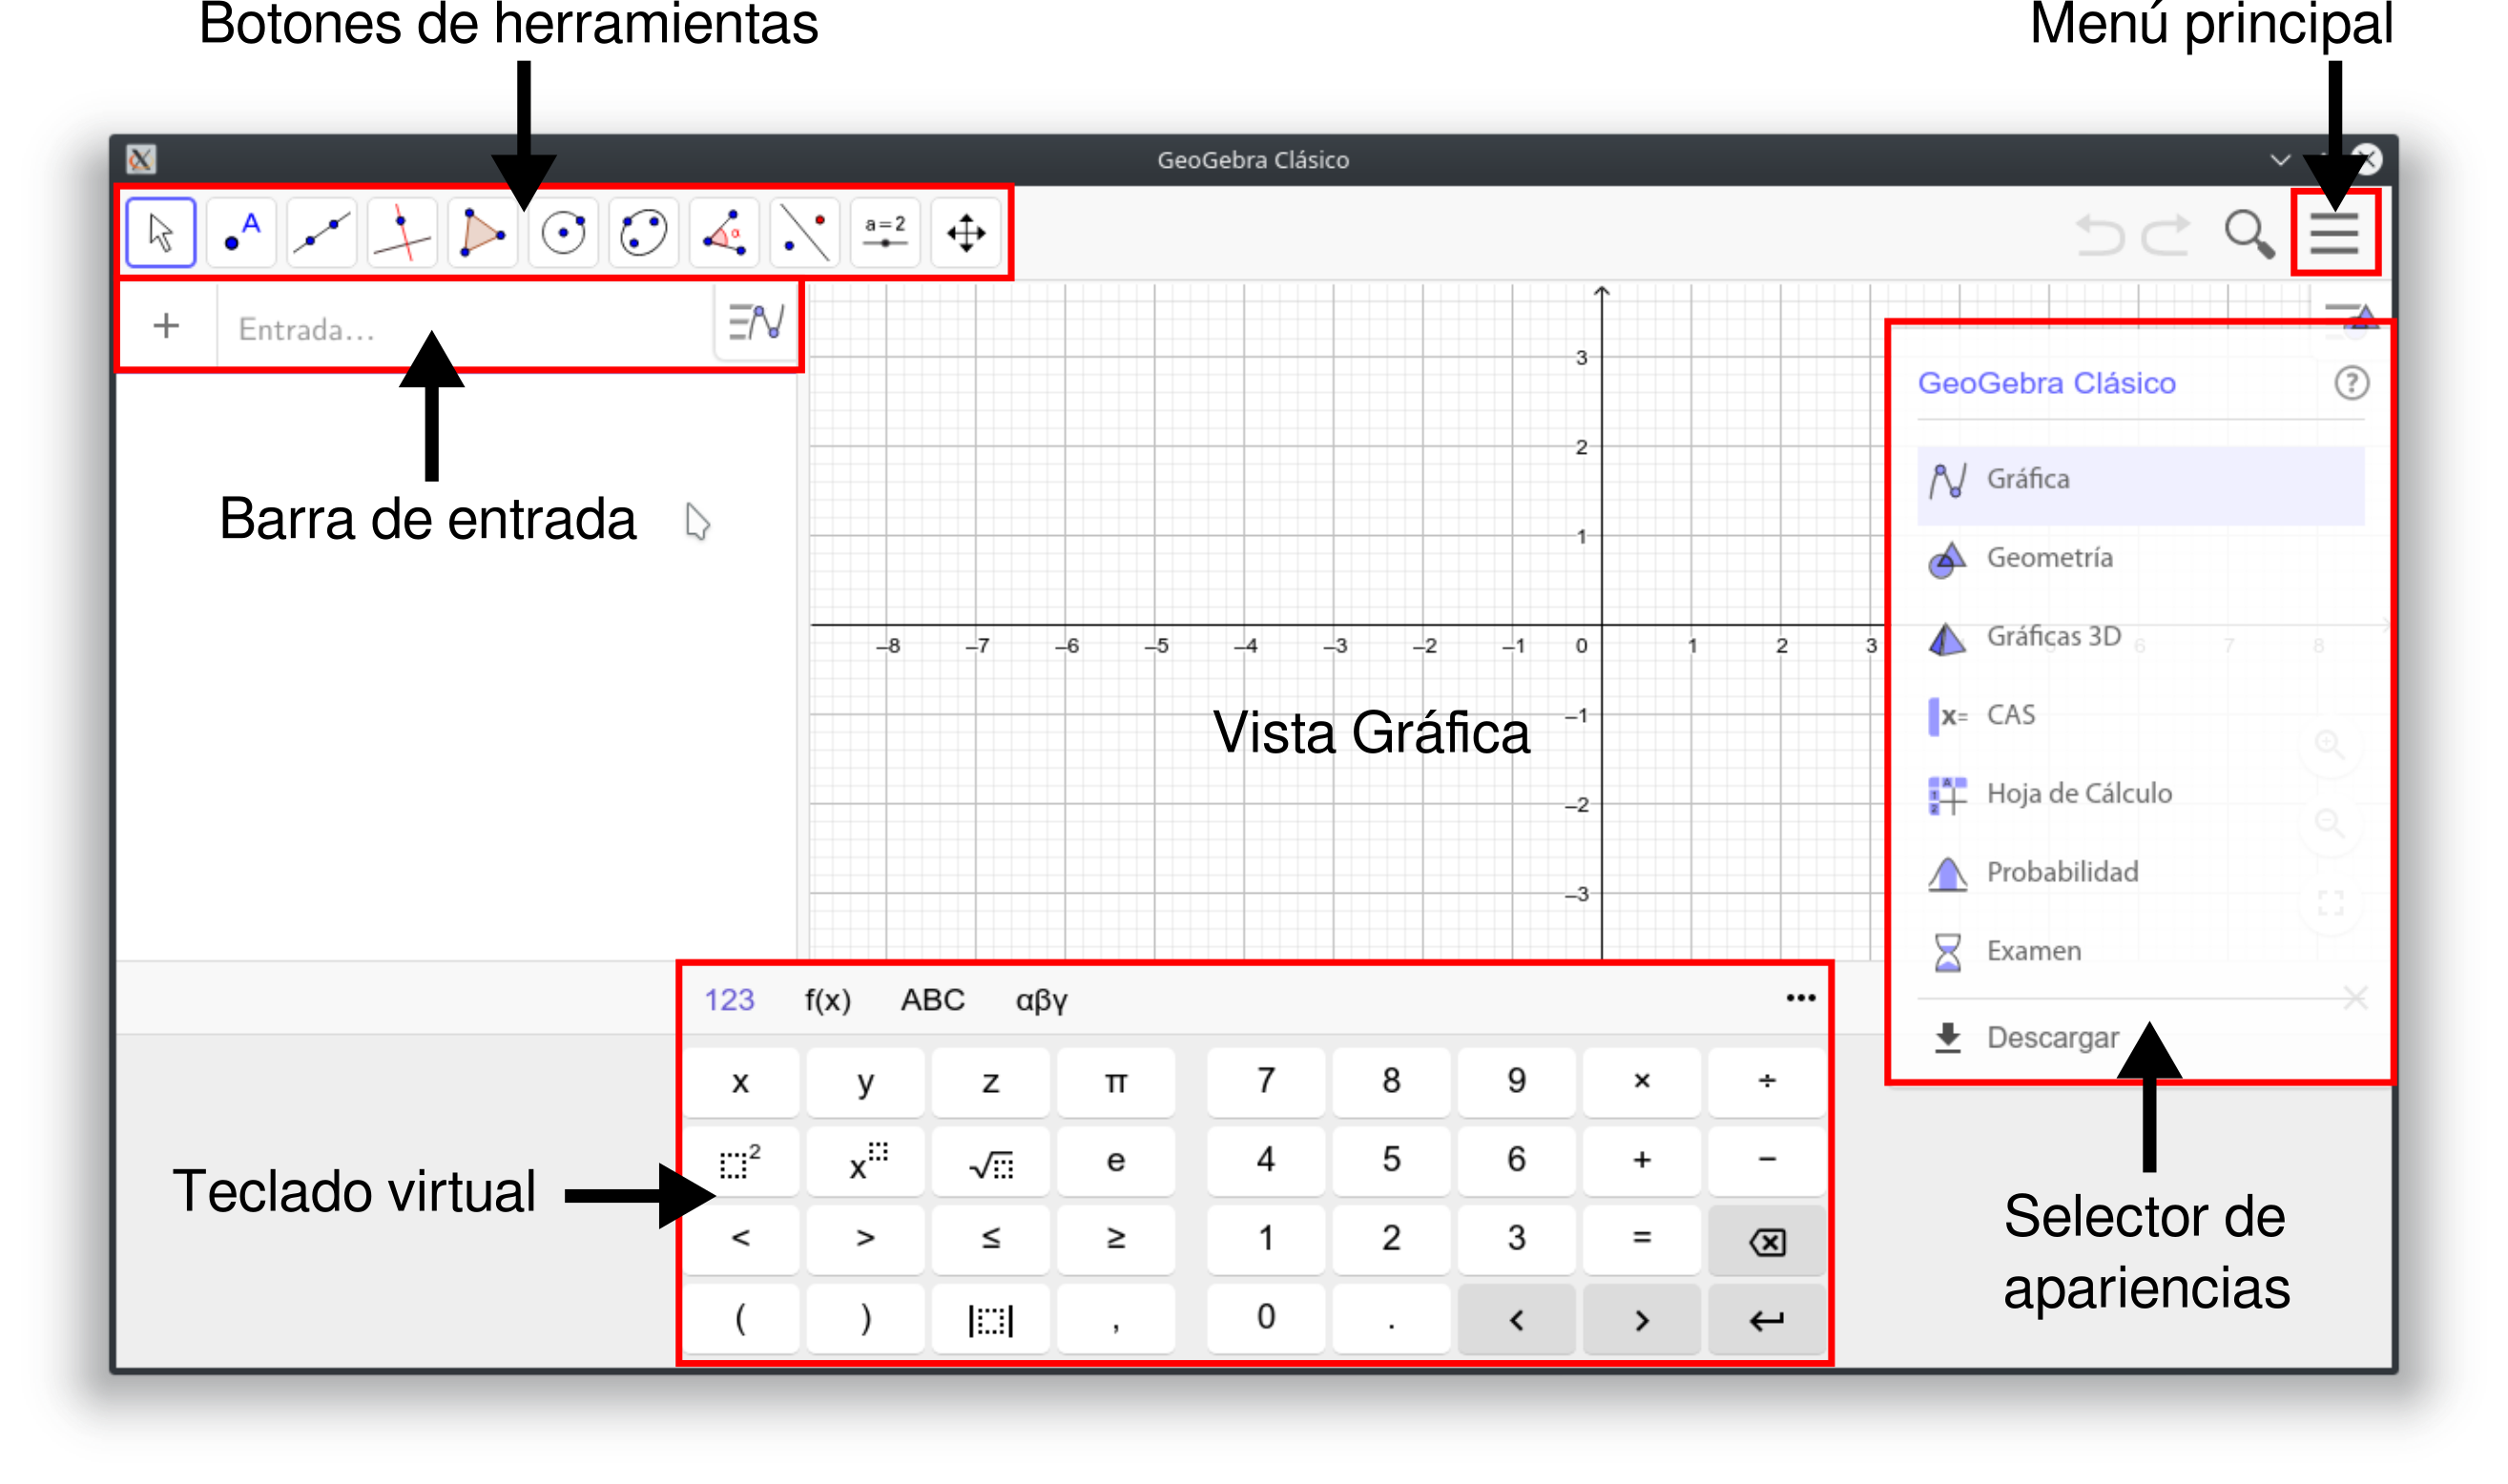
\includegraphics[width=\textwidth]{img/introduccion/start-window}
\caption{Ventana principal de Geogebra.} \label{g:ventana-inicio}
\end{center}
\end{figure}

\section{Vistas}
Geogebra dispone de varias ventanas de trabajo que se denominan \emph{Vistas} y de distintos entornos de trabajo llamados \emph{Apariencias} que combinan distintas vistas.
Tanto las vistas como las apariencias se pueden activar en el menú principal de Geogebra que aparece en la esquina superior derecha.
Las vistas más importantes que utilizaremos a lo largo de estas prácticas son:
\begin{description}
\item[Vista Algebraica] 
\includegraphics[scale=0.03]{img/introduccion/algebraic-view-icon} Esta permite realizar construcciones algebraicas y geométricas.
      Dispone una \field{Barra de Entrada} donde se pueden introducir comandos y expresiones algebraicas.
      Esta vista aparece activa por defecto cuando arranca el programa.
\item[Vista Gráfica] 
\includegraphics[scale=0.03]{img/introduccion/graphics-view-icon} Esta vista permite representar objetos geométricos en el plano real.
      Junto a la vista algebraica, esta vista también aparece activa por defecto cuando arranca el programa.
\item[Vista Gráfica 3D] 
\includegraphics[scale=0.3]{img/introduccion/3d-graphics-view-icon} Esta vista permite representar objetos geométricos en el espacio real.
      Esta vista no aparece por defecto cuando arranca el programa, así que hay que activarla cuando se necesite.
\item[Vista CAS] 
\includegraphics[scale=0.03]{img/introduccion/cas-view-icon} (Computer Algebra System) Esta vista permite realizar cálculos simbólicos. Dispone de una \field{Barra de Entrada} similar a la vista Algebraica donde se pueden introducir comandos y expresiones matemáticas y evaluarlas.
      Esta vista no aparece por defecto cuando arranca el programa, pero \emph{será la que más utilizaremos durante las prácticas.}
\end{description}


\section{Edición de expresiones en la \field{Vista CAS}}
Antes de realizar cualquier cálculo sobre una expresión matemática, lo primero es escribir dicha expresión y aprender a manipularla.


\subsection*{Introducción de expresiones}
Para introducir una expresión se utiliza \field{Barra de Entrada} de la \field{Vista CAS} (figura~\ref{g:barra-entrada}).

\begin{figure}[h!]
\begin{center}

\includegraphics[scale=0.6]{img/introduccion/input-bar}
\caption{Barra de entrada de expresiones.} \label{g:barra-entrada}
\end{center}
\end{figure}

La \field{Barra de Entrada} permite introducir expresiones matemáticas, comandos y también anotaciones de texto.
En estas expresiones podemos introducir números, letras romanas, letras griegas, operadores matemáticos y cualquier símbolo matemático que aparece en el teclado virtual.
También permite la entrada de código \LaTeX\footnote{\url{https://www.latex-project.org/}} para formatear la expresiones.

Cuando se presiona la tecla \command{Enter} después de introducir una expresión matemática, Geogebra trata de evaluarla y muestra el resultado de la evaluación justo debajo de la expresión, o bien un aviso de error cuando hay algo mal escrito en la expresión.

Los operadores más habituales en la construcción de expresiones son los que aparecen en la siguiente tabla:

\begin{center}
\begin{tabular}{cc}
\tcrule
\textbf{Símbolo} & \textbf{Operador} \\
\texttt{+}       & suma              \\
\texttt{-}       & resta             \\
\texttt{*}       & producto          \\
\texttt{/}       & división          \\
\texttt{\^{}}    & potencia          \\
\bcrule
\end{tabular}
\end{center}

A la hora de escribir una expresión hay que tener en cuenta que Geogebra tiene establecido un orden de prioridad en la evaluación de los operadores.
En primer lugar evalúa las funciones y constantes predefinidas, después evalúa las potencias, después productos y cocientes (ambos con igual prioridad y de izquierda a derecha), y por último sumas y restas (ambas con igual prioridad y de izquierda a derecha).
Para forzar la evaluación de una subexpresión, saltándose el orden de prioridad, se utilizan paréntesis.
Así, como se ve en el siguiente ejemplo, dependiendo de cómo se introduzca una expresión pueden obtenerse resultados diferentes.


\begin{center}\renewcommand{\arraystretch}{2}
\begin{tabular}{cc}
\tcrule
\textbf{Expresión introducida} & \textbf{Expresión evaluada} \\
\texttt{4x-1/x-5}              & $4x-\dfrac{1}{x}-5$         \\
\texttt{(4x-1)/x-5}            & $\dfrac{4x-1}{x}-5$         \\
\texttt{4x-1/(x-5)}            & $4x-\dfrac{1}{x-5}$         \\
\texttt{(4x-1)/(x-5)}          & $\dfrac{4x-1}{x-5}$         \\
\bcrule
\end{tabular}
\end{center}

Cada vez que introducimos una expresión, esta aparece en la \field{Vista CAS} etiquetada con un número que permite identificarla.
Posteriormente, cada vez que queramos hacer referencia a dicha expresión podremos utilizar su identificador en lugar de volver a escribir la expresión.

Existen dos formas de referirse a una expresión anterior, que son la referencia estática y la referencia dinámica.
Para hacer una referencia estática debemos escribir el símbolo \# seguido el número que identifica la expresión, mientas que para hacer una referencia dinámica debemos escribir el símbolo \$ seguido del número que identifica la expresión.
Una referencia estática no cambiará la expresión donde se hace la referencia aún cuando la expresión original cambie, mientras que en una referencia dinámica, cuando cambie la expresión original, la expresión donde se hace la referencia reflejará ese cambio.

Es posible seleccionar cualquier expresión o subexpresión de la \field{Vista CAS} y copiarla y pegarla en la \field{Barra de Entrada}.


\subsection*{Introducción de anotaciones de texto}
Geogebra permite también la introducción de anotaciones o comentarios de texto en la \field{Barra de Entrada}.
Para ello hay que hacer clic con el botón derecho del ratón en la \field{Barra de Entrada} y seleccionar el menú \menu{Texto} del menú contextual que aparece.
Las anotaciones de texto son muy útiles para explicar los pasos que se dan en una construcción matemática o para interpretar los resultados.


\subsection*{Eliminación de expresiones}
Por supuesto, es posible eliminar una expresión de la \field{Vista CAS}.
Para ello solo hay que ir a la línea que contiene la expresión que se quiere eliminar y hacer clic en el botón 
\includegraphics[scale=0.035]{img/introduccion/bin-button.png} o hacer clic con el botón derecho del ratón y seleccionar el menú \menu{Eliminar fila} del menú contextual que aparece.

Si cometemos un error introduciendo una expresión o eliminándola, es posible deshacer las últimas operaciones o rehacerlas haciendo clic sobre los botones 
\includegraphics[scale=0.03]{img/introduccion/undo-button.png} o 
\includegraphics[scale=0.03]{img/introduccion/redo-button.png} respectivamente.


\subsection*{Definición de variables}
Para definir variables se pueden utilizar letras romanas o griegas.
Geogebra permite definir variables de más de una letra, de manera que la expresión \texttt{xy}, no se interpreta como el producto de la variable $x$ por la variable $y$, sino como la variable $xy$.
Además, distingue entre mayúsculas y minúsculas, así que no es lo mismo $xy$ que $xY$.


\subsection*{Definición de constantes y funciones}
Es posible definir constantes y funciones mediante el operador de definición \command{:=}.
Para definir una constante basta con escribir el nombre de la constante seguido de \command{:=} y el valor de dicha constante.
Por ejemplo para definir la constante de la aceleración de la gravedad, escribiríamos \command{g:=9.81}.

Por otro lado, para definir una función se escribe el nombre de la función seguido de la lista de variables de la misma separadas por comas y entre paréntesis; después se escribe \command{:=} y por último la expresión que define la función.
Así, por ejemplo, para definir la función que calcula el área de un triángulo de base $b$ y altura $h$, escribiríamos \command{a(b,h):=(b*h)/2} (ver figura~\ref{g:expresiones}).

Si hemos definido una función o una constante, y posteriormente cambiamos la definición, los cambios se verán reflejados en cualquier expresión donde aparezca la constante o la función, a no ser que hayamos hecho una referencia estática a ella.

Para eliminar la definición y dejar libre el nombre de la constante o función, por ejemplo \command{c}, se puede utilizar el comando \command{Eliminar(c)} o bien el comando \command{c:=}.

\subsection*{Funciones y constantes predefinidas}
Geogebra tiene ya predefinidas la mayoría de la funciones elementales y constantes que suelen utilizarse en los cálculos matemáticos.
La sintaxis de algunas de estas funciones y constantes se muestra en la tabla~\ref{t:funciones-predefinidas}, aunque, muy a menudo, en lugar de utilizar dicha sintaxis se utilizan los operadores y constantes que aparecen en el teclado virtual.

\begin{table}[h!]
\centering
\begin{tabular}{cl}
\tcrule
\textbf{Sintaxis}   & \textbf{Constante o función}                 \\
\command{pi}        & El número $\pi=3.14159\ldots$                \\
\command{Alt+e}     & Constante de Euler $e=2.71828\ldots$         \\
\command{Alt+i}     & El número imaginario $i=\sqrt{-1}$           \\
\command{inf}       & Infinito $\infty$                            \\
\command{exp(x)}    & Función exponencial $e^x$                    \\
\command{log(a,x)}  & Función logarítmica con base $a$, $\log_a x$ \\
\command{ln(x)}     & Función logaritmo neperiano $\ln x$          \\
\command{sqrt(x)}   & Función raíz cuadrada $\sqrt{x}$             \\
\command{sen(x)}    & Función seno $\sin x$                        \\
\command{cos(x)}    & Función coseno $\cos x$                      \\
\command{tan(x)}    & Función tangente $\tan x$                    \\
\command{arcsin(x)} & Función arcoseno $\arcsin x$                 \\
\command{arccos(x)} & Función arcocoseno $\arccos x$               \\
\command{arctan(x)} & Función arcotangente $\arctan x$             \\
\bcrule
\end{tabular}
\caption{Sintaxis de algunas funciones elementales y constantes predefinidas en Geogebra.} \label{t:funciones-predefinidas}
\end{table}

\subsection*{Vectores y matrices}
Geogebra también permite la manipulación de vectores y matrices.
Para definir un vector se escriben sus coordenadas separadas por comas entre paréntesis.
Por ejemplo, para introducir el vector $(x,y,z)$ escribiríamos \command{(x,y,z)} (ver figura~\ref{g:expresiones}).
Si se quiere un vector columna se puede usar el comando \command{Vector((x,y,z))}.

Para definir una matriz se escriben sus elementos por filas, separados por comas y entre llaves.
Así, para introducir por ejemplo la matriz
\[
\left(
\begin{array}{ccc}
1 & 2 & 3 \\
a & b & c \\
\end{array}
\right)
\]
escribiríamos \command{\{\{1,2,3\},\{a,b,c\}\}} (ver figura~\ref{g:expresiones}).


\subsection*{Simplificación de expresiones}
Geogebra trata de simplificar las expresiones cuando las evalúa.
Por ejemplo, si se introduce $x+x$ el resultado será $2x$.
Si no se desea evaluar una expresión se puede cambiar al modo de conservar las entradas haciendo clic en el botón 
\includegraphics[scale=0.03]{img/introduccion/keep-input-button}.

Sin embargo al evaluar una expresión Geogebra no realiza simplificaciones más complejas como por ejemplo simplificar la expresión $\sen(x)^2+\cos(x)^2=1$.
Para ello dispone de tres comandos:
\begin{description}
\item[Simplifica] Es el comando más sencillo y trata de simplificar al máximo una función.
      Por ejemplo, el comando \command{Simplifica(sen(x)\^{}2+cos(x)\^{}2)} devolverá \result{1}.
\item[Desarrolla] Este comando permite desarrollar una expresión realizando los potencias, productos, cocientes, sumas y restas que se puedan.
      Por ejemplo, el comando \command{Desarrolla((x+1)\^{}2)} devolverá el resultado \result{x\^{}2+2x+1}.
\item[Factoriza] Este comando permite factorizar una expresión.
      Por ejemplo, el comando \command{Factoriza(x\^{}2+2x+1)} devolverá el resultado \result{(x+1)\^{}2}.
\end{description}

En cualquiera de estas simplificaciones, Geogebra trabaja por defecto en modo exacto y por eso devuelve expresiones fraccionarias.
Para obtener el valor de una expresión en modo aproximado, con decimales, hay que cambiar al modo de cálculo aproximado haciendo clic sobre el botón 
\includegraphics[scale=0.03]{img/introduccion/approximate-button}.
El número de cifras decimales se puede establecer en la configuración de Geogebra.

Por último, es posible sustituir cualquier variable de una expresión por un valor u otra expresión mediante el comando \command{Sustituye(<expresion>, <Lista de reemplazos>)}.
Por ejemplo, el comando \command{Sustituye(2x+y, x=2, y=1)} devolverá el resultado \result{5}.

\subsection*{Ecuaciones e inecuaciones}
Para definir ecuaciones en Geogebra hay que utilizar el símbolo de igualdad \command{=}.
Por ejemplo, el comando \command{2x-y=1} define la ecuación de una recta.

Y para definir inecuaciones en Geogebra hay que utilizar los símbolos de menor \command{<}, mayor \command{>}, menor o igual \command{<=} o mayor o igual \command{>=}.
Por ejemplo, el comando \command{x\^{}2+y\^{}2<=1} define el círculo de radio 1 centrado en el origen.

Para resolver ecuaciones e inecuaciones se utiliza el comando \command{Resuelve(<ecuaciones>)}.
Por ejemplo, el comando \command{Resuelve(x\^{}2-5x+4=0)} devolverá el resultado \result{\{x=1, x=4\}}.
Se pueden indicar además restricciones para las variables.
Por ejemplo, el comando \command{Resuelve(x\^{}2-5x+4=0, x>3)} devolverá únicamente la solución \result{\{x=4\}}.

Para resolver sistemas de ecuaciones hay que poner la lista de ecuaciones entre llaves.
Por ejemplo, el comando \command{Resuelve({2x+3=7, x-y=-1})} devolverá el resultado \result{\{x=3, y=2\}}.

Este comando también permite resolver inecuaciones.
Por ejemplo, el comando \command{Resuelve(3x-2<1)} devolverá el resultado \result{\{x<1\}}.


\section{Representaciones gráficas}
Uno de los puntos fuertes de Geogebra es su capacidad gráfica ya que permite representar multitud de objetos geométricos tanto en el plano como en el espacio real.

\subsection*{Representaciones gráficas en el plano real}
Para representar objetos geométricos en el plano real $\mathbb{R}^2$, Geogebra dispone de la \field{Vista Gráfica}.
Por defecto cualquier función que definamos en la \field{Vista CAS} aparecerá representada en esta vista.
Para representar otros objetos como constantes, ecuaciones o inecuaciones es necesario hacer clic sobre el círculo que aparece a la izquierda de la expresión (ver figura~\ref{g:vista-grafica}).
Para ocultar de nuevo el objeto en la \field{Vista Gráfica} basta con volver a hacer clic sobre ese círculo.

\begin{figure}[h!]
\begin{center}
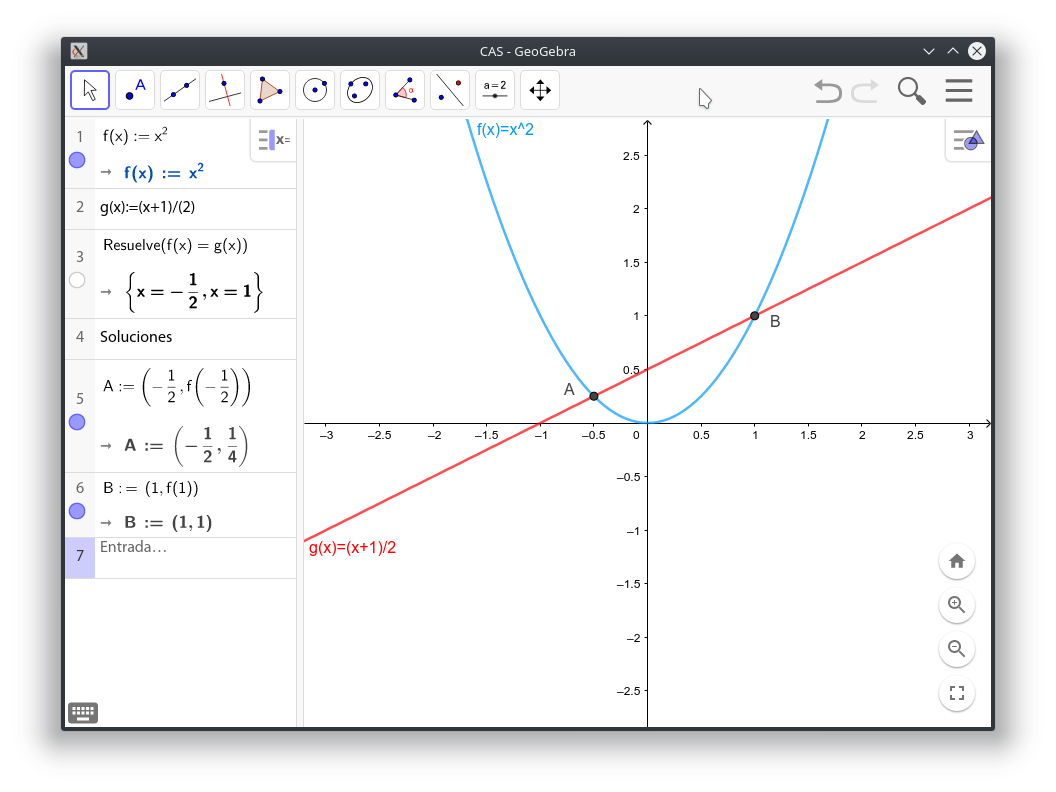
\includegraphics[width=\textwidth]{img/introduccion/graphic-view}
\caption{Representaciones gráficas en la \field{Vista Gráfica}.} \label{g:vista-grafica}
\end{center}
\end{figure}

Geogebra permite también la representación de curvas paramétricas utilizando el comando \command{Curva(<Expresión>, <Expresión>, <Parámetro>, <Valor inicial>, <Valor final>)}, donde las dos primeras expresiones dan las coordenadas $x$ e $y$ de la curva en función del parámetro.
Por ejemplo, el comando \command{Curva(cos(t), 2sen(t)cos(t), t, 0, 2pi)} dibuja la curva que se muestra en la figura~\ref{g:curva-parametrica}.

\begin{figure}[h!]
\begin{center}
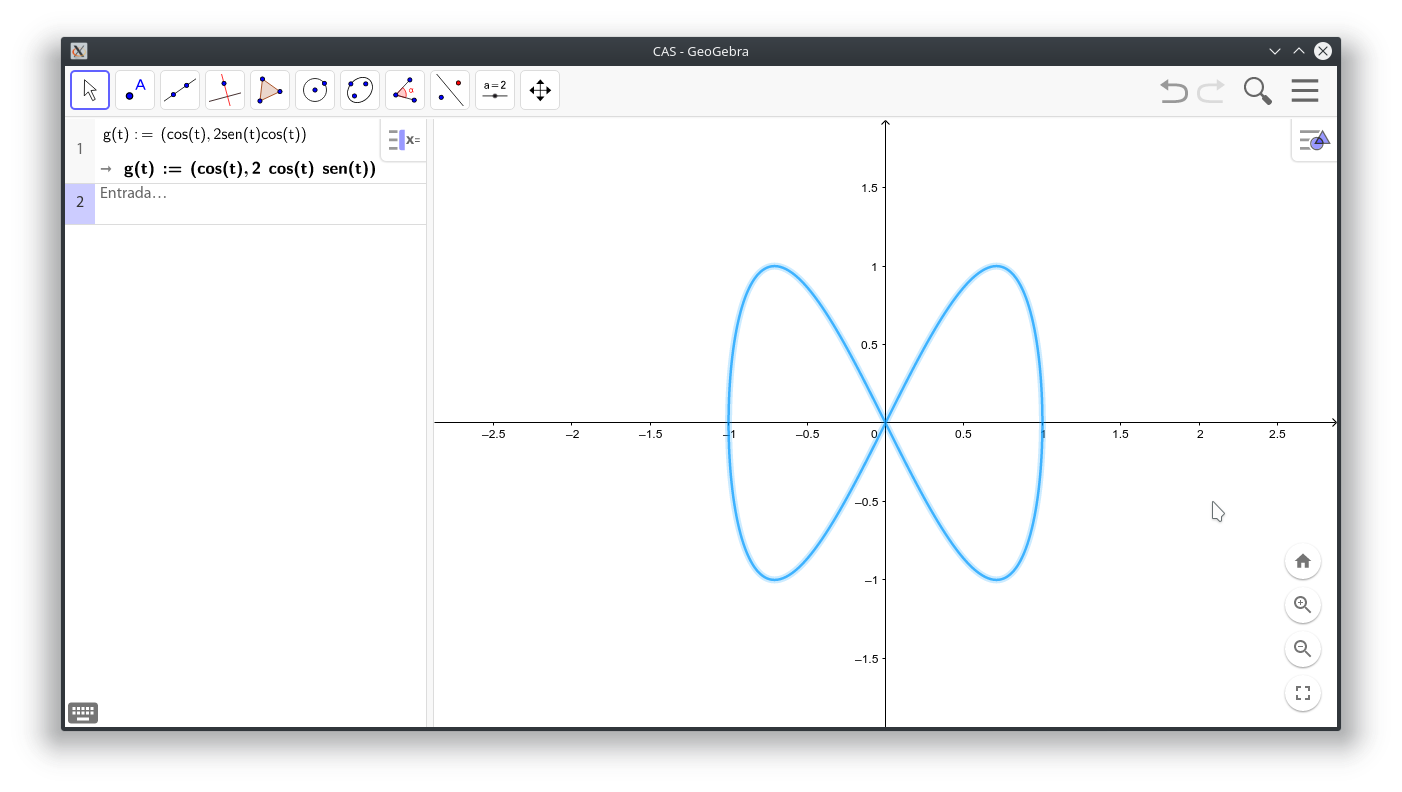
\includegraphics[width=\textwidth]{img/introduccion/parametric-curve}
\caption{Representación de una curva paramétrica en el plano.} \label{g:curva-parametrica}
\end{center}
\end{figure}

Es posible cambiar el aspecto de cualquier objeto geométrico haciendo clic con el botón derecho del ratón sobre él y seleccionando el menú \menu{Configuración} del menú contextual que aparece.
Esto abre un panel que permite cambiar el nombre del objeto, el color, el grosor o la transparencia del trazo, e incluso ponerle un rótulo que aparezca en la \field{Vista Gráfica} junto al objeto.

La \field{Vista Gráfica} aparece centrada en el origen de coordenadas por defecto, pero se puede hacer un zoom para acercar o alejar la vista haciendo clic en los botones 
\includegraphics[scale=0.03]{img/introduccion/zoom-in-button} y 
\includegraphics[scale=0.03]{img/introduccion/zoom-out-button} respectivamente.
También es posible desplazar la vista haciendo clic en cualquier posición y, sin soltar, desplazando el ratón.
Para volver a la vista original centrada en el origen de coordenadas, basta con hacer clic en el botón 
\includegraphics[scale=0.03]{img/introduccion/home-button}.


\subsection*{Representaciones gráficas en el espacio real}
Para representar objetos geométricos en el espacio real $\mathbb{R}^3$, Geogebra dispone de la \field{Vista Gráficas 3D}.

Por defecto cualquier función de dos variables que definamos en la \field{Vista CAS} aparecerá representada en esta vista.
Para representar otros objetos como ecuaciones es necesario hacer clic sobre el círculo que aparece a la izquierda de la expresión (ver figura~\ref{g:vista-grafica-3D}).
Para ocultar de nuevo el objeto en la \field{Vista Gráfica} basta con volver a hacer clic sobre ese círculo.

\begin{figure}[h!]
\begin{center}
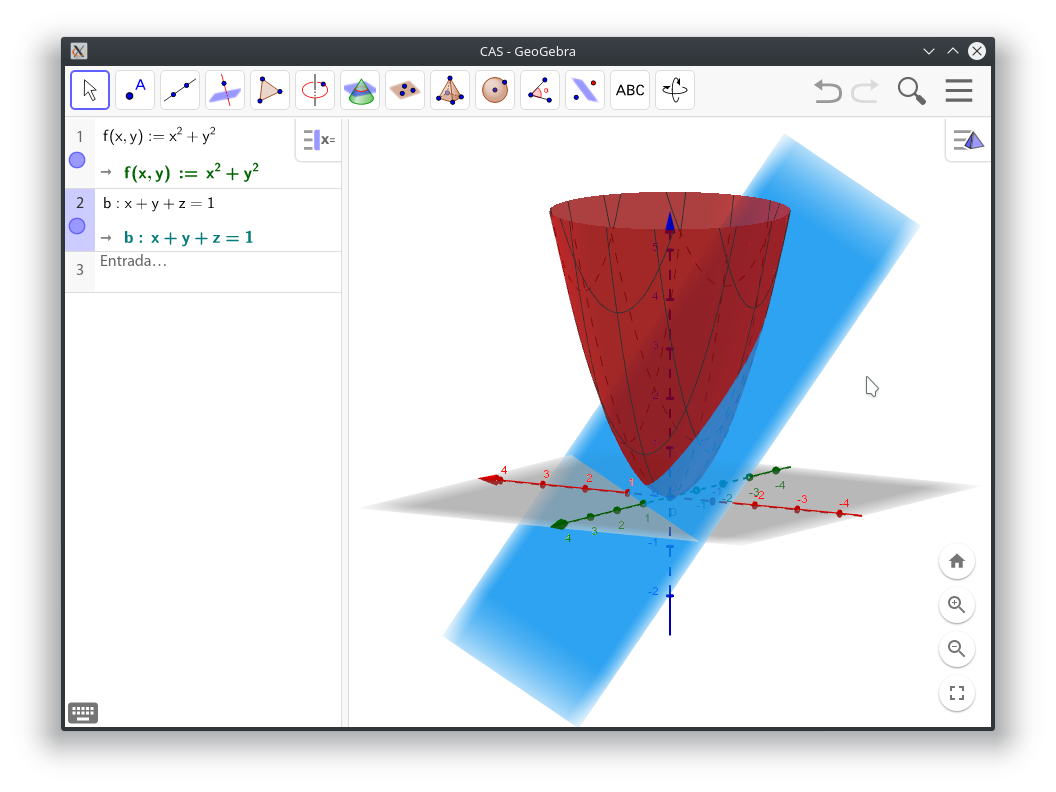
\includegraphics[width=\textwidth]{img/introduccion/3D-graphic-view}
\caption{Representaciones gráficas en la \field{Vista Gráfica 3D}.} \label{g:vista-grafica-3D}
\end{center}
\end{figure}

También es posible la representación de curvas paramétricas utilizando el comando \command{Curva(<Expresión>, <Expresión>, <Expresión>, <Parámetro>, <Valor inicial>, <Valor final>)}, donde las tres primeras expresiones dan las coordenadas $x$, $y$ y $z$ de la curva en función del parámetro.
Por ejemplo, el comando \command{g(t):=Curva(cos(t), sen(t), t/2, t, 0, 2pi)} dibuja la curva que se muestra en la figura~\ref{g:curva-parametrica-3D}.

\begin{figure}[h!]
\begin{center}
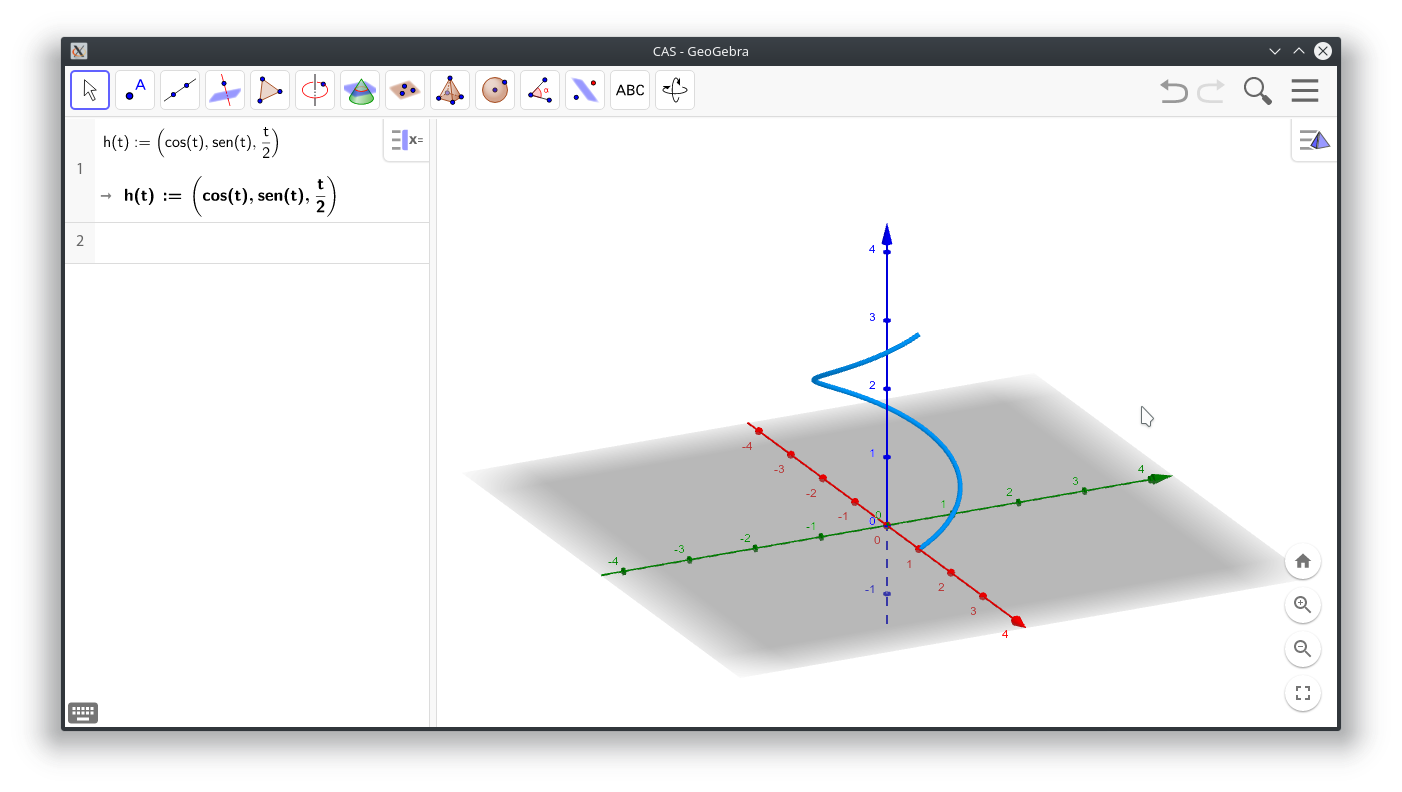
\includegraphics[width=\textwidth]{img/introduccion/3D-parametric-curve}
\caption{Representación de una curva paramétrica en el espacio.} \label{g:curva-parametrica-3D}
\end{center}
\end{figure}

Al igual que en la \field{Vista Gráfica}, es posible cambiar el aspecto de cualquier objeto geométrico haciendo clic con el botón derecho del ratón sobre él y seleccionando el menú \menu{Configuración} del menú contextual que aparece.
Esto abre un panel que permite cambiar el nombre del objeto, el color, el grosor o la transparencia del trazo, e incluso ponerle un rótulo que aparezca en la \field{Vista Gráfica} junto al objeto.

Del mismo modo, es posible hacer un zoom para acercar o alejar la vista haciendo clic en los botones 
\includegraphics[scale=0.03]{img/introduccion/zoom-in-button} y 
\includegraphics[scale=0.03]{img/introduccion/zoom-out-button} respectivamente.
También se puede mover la vista con el botón 
\includegraphics[scale=0.03]{img/introduccion/move-button} o rotarla con el botón 
\includegraphics[scale=0.03]{img/introduccion/rotate-button}.


\section{Gestión de archivos}
Las expresiones y los cálculos realizados dentro de la \field{Vista CAS} se pueden guardar en un archivo.

\subsection*{Guardar un archivo}
Para guardar las expresiones y los resultados de la \field{Vista CAS} se puede utiliza el menú \menu{Archivo>Guardar}.
Si no hemos iniciado sesión en el servidor de Geogebra nos preguntará el nombre de usuario y la contraseña para iniciar la sesión (ver figura~\ref{g:login}).
Si aún no se dispone de una cuenta de usuario es posible registrarse también en este momento, pero si no se desea identificarse se puede hacer clic en el enlace \command{Continuar sin identificarse ahora}.

\begin{figure}[h!]
\begin{center}
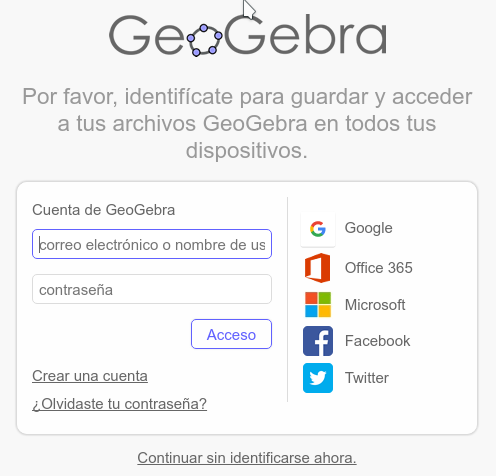
\includegraphics[scale=0.6]{img/introduccion/login}
\caption{Inicio de sesión en el servidor de Geogebra} \label{g:login}
\end{center}
\end{figure}

Si hemos iniciado sesión en el servidor, nos preguntará el nombre que queremos darle al archivo y se subirá automáticamente a la nube de Geogebra.
De este modo estará disponible en la web de Geogebra cuando nos conectemos con nuestro cuenta de usuario.

Si no se ha iniciado sesión en el servidor, entonces aparecerá un cuadro de diálogo donde podremos indicar el nombre que queremos darle al fichero y la seleccionar la carpeta donde queremos guardarlo.
Los archivos de geogebra tienen extensión \texttt{*.ggb}.

Una vez guardado el archivo, su nombre aparecerá en la barra de título de la ventana de Geogebra.


\subsubsection*{Abrir un archivo}
Para abrir un archivo de geogebra se utiliza el \menu{Archivo>Abrir}.
En el cuadro de diálogo que aparece se puede optar por abrir un archivo de la web de Geogebra, o bien abrir un archivo local.

En el caso de que hayamos iniciado sesión en el servidor, automáticamente aparecerán nuestros archivos de la nube de Geogegra.
Si no hemos iniciado sesión en el servidor entonces se puede abrir cualquier archivo público de la web de Geogebra.
Para ello podemos introducir cualquier término en la barra de búsqueda que aparece y nos aparecerán los archivos que incluyen esos términos.
Seleccionando cualquiera de ellos se descargará y se abrirá en Geogebra.

Si se desea abrir un archivo local hay que hacer clic en la carpeta que aparece y se abrirá un cuadro de diálogo donde debemos indicar el archivo que queremos abrir.


\section{Impresión}
Geogebra permite imprimir las vistas gráficas seleccionando el menú \menu{Previsualización}.
Tras esto aparece un cuadro de diálogo donde se puede seleccionar la ventana gráfica que se desea imprimir y las unidades de los ejes.
Finalmente aparece el cuadro de diálogo de las impresoras donde hay que seleccionar la impresora con la que se quiere imprimir.

También es posible exportar las vistas gráficas a diferentes formatos con el menú \menu{Descargar como}.
Si se desea imprimir además de las gráficos las expresiones de la \field{Vista CAS} hay que seleccionar la opción \option{Construcción dinámica con página web (html)}.
Esto genera una página web que puede abrirse con cualquier navegador y después imprimirse de la forma habitual.


\section{Ejercicios resueltos}
\begin{enumerate}
\item Introducir y evaluar las siguientes expresiones matemáticas.
      \begin{enumerate}
      \item $4x-\dfrac{1}{x}-5$.
            \begin{indication}
            Introducir la expresión \command{4x-1/x-5} en la \field{Barra de Entrada} de la \field{Vista CAS}.
            \end{indication}
      \item $\dfrac{4x-1}{x}-5$.
            \begin{indication}
            Introducir la expresión \command{(4x-1)/x-5} en la \field{Barra de Entrada} de la \field{Vista CAS}.
            \end{indication}
      \item $4x-\dfrac{1}{x-5}$.
            \begin{indication}
            Introducir la expresión \command{4x-1/(x-5)} en la \field{Barra de Entrada} de la \field{Vista CAS}.
            \end{indication}
      \item $\dfrac{4x-1}{x-5}$.
            \begin{indication}
            Introducir la expresión \command{(4x-1)/(x-5)} en la \field{Barra de Entrada} de la \field{Vista CAS}.
            \end{indication}
      \end{enumerate}

\item Definir las siguientes objetos matemáticos y dibujarlos.
      \begin{enumerate}
      \item Las constantes $a=2$ y $b=3$.
            \begin{indication}
            \begin{enumerate}
            \item Introducir el comando \command{a:=2} en la \field{Barra de Entrada} de la \field{Vista CAS} y activar la \field{Vista Gráfica}.
            \item Para dibujar el deslizador de la constante hacer clic sobre el círculo que aparece a la izquierda de la expresión anterior.
            \item Introducir el comando \command{b:=3} en la \field{Barra de Entrada}.
            \item Para dibujar el deslizador de la constante hacer clic sobre el círculo que aparece a la izquierda de la expresión anterior.
            \end{enumerate}
            \end{indication}
      \item La recta $f(x)=a+bx$.
            Utilizar los deslizadores de las constantes para ver cómo cambia la recta.
            \begin{indication}
            Introducir el comando \command{f(x):=a+b*x} en la \field{Barra de Entrada}.
            \end{indication}
      \item La ecuación $ax^2+by^2=8$.
            Utilizar los deslizadores de las constantes para ver cómo cambia la recta.
            \begin{indication}
            Introducir el comando \command{a*x\^{}2+b*y\^{}2=8} en la \field{Barra de Entrada}.
            \end{indication}
      \end{enumerate}
\end{enumerate}
% !TEX root = ../practicas_geogebra.tex
% Author: Alfredo Sánchez Alberca (asalber@ceu.es)
\chapter{Funciones Elementales}

% \section{Fundamentos teóricos}

% En esta práctica se introducen los conceptos básicos sobre funciones reales de variable real, esto es, funciones
% \[f:\mathbb{R}\rightarrow \mathbb{R}.\]

% \subsection{Dominio e imagen}

% El \emph{Dominio} de la función $f$ es el conjunto de los números reales $x$ para los que existe $f(x)$ y se designa mediante $\dom f$.

% La \emph{Imagen} de $f$ es el conjunto de los números reales $y$ para los que existe algún $x\in \mathbb{R}$ tal que $f(x)=y$, y se denota por $\im f$.


% \subsection{Signo y crecimiento}
% El \emph{signo} de la función es positivo $(+)$ en los valores de $x$ para los que $f(x)>0$ y negativo $(-)$ en los que $f(x)<0$.
% Los valores de $x$ en los que la función se anula se conocen como \emph{raíces} de la función.

% Una función $f(x)$ es \emph{creciente} en un intervalo $I$ si $\forall\, x_1, x_2 \in I$ tales que $x_1<x_2$ se verifica que $f(x_1)\leq f(x_2)$.

% Del mismo modo, se dice que una función $f(x)$ es \emph{decreciente} en un intervalo $I$ si $\forall\, x_1, x_2 \in I$ tales que $x_1<x_2$ se verifica que $f(x_1)\geq f(x_2)$. En la figura~\ref{g:crecimiento} se muestran estos conceptos.

% \begin{figure}[h!]
% 	\centering \subfigure[Función creciente.] {\label{g:funcion_creciente}
% 		\scalebox{1}{\input{img/funciones_elementales/funcion_creciente}}}\qquad
% 	\subfigure[Función decreciente.]{\label{g:funcion_decreciente}
% 		\scalebox{1}{\input{img/funciones_elementales/funcion_decreciente}}}
% 	\caption{Crecimiento de una función.}
% 	\label{g:crecimiento}
% \end{figure}


% \subsection{Extremos Relativos}
% Una función $f(x)$ tiene un \emph{máximo relativo} en $x_0$ si existe un entorno $A$ de $x_0$ tal que $\forall x \in A$
% se verifica que $f(x)\leq f(x_0)$.

% Una función $f(x)$ tiene un \emph{mínimo relativo} en $x_0$ si existe un entorno $A$ de $x_0$ tal que $\forall x\in A$
% se verifica que $f(x)\geq f(x_0)$.

% Diremos que la función $f(x)$ tiene un \emph{extremo relativo} en un punto si tiene un \emph{máximo o mínimo relativo}
% en dicho punto. Estos conceptos se muestran en la figura~\ref{g:extremos}.

% \begin{figure}[h!]
% 	\centering \subfigure[Máximo relativo.] {\label{g:maximo}
% 		\scalebox{1}{\input{img/funciones_elementales/maximo}}}\qquad
% 	\subfigure[Mínimo relativo.]{\label{g:minimo}
% 		\scalebox{1}{\input{img/funciones_elementales/minimo}}}
% 	\caption{Extremos relativos de una función.}
% 	\label{g:extremos}
% \end{figure}

% Una función $f(x)$ está \emph{acotada superiormente} si $\exists K\in\mathbb{R}$ tal que $f(x)\leq K$ $\forall x \in \dom f$. Análogamente, se dice que una función $f(x)$ está \emph{acotada inferiormente} si $\exists K\in\mathbb{R}$ tal que $f(x)\geq K$ $\forall x \in \dom f$.

% Una función $f(x)$ está \emph{acotada} si lo está superior e inferiormente, es decir si $\exists K\in\mathbb{R}$ tal que $|f(x)|\leq K$ $\forall x \in \dom f$.


% \subsection{Concavidad}

% De forma intuitiva se puede decir que una función $f(x)$ es \emph{cóncava} en un intervalo $I$ si $\forall\, x_1, x_2
% \in I$, el segmento de extremos $(x_1,f(x_1))$ y $(x_2,f(x_2))$ queda por encima de la gráfica de $f$.

% Análogamente se dirá que es \emph{convexa} si el segmento anterior queda por debajo de la gráfica de $f$.

% Diremos que la función $f(x)$ tiene un \emph{punto de inflexión} en $x_0$ si en ese punto la función pasa de cóncava a
% convexa o de convexa a cóncava. Estos conceptos se ilustran en la figura~\ref{g:concavidad}.

% \begin{figure}[h!]
% 	\centering \subfigure[Función cóncava.] {\label{g:funcion_convexa}
% 		\scalebox{1}{\input{img/funciones_elementales/funcion_convexa}}}\qquad
% 	\subfigure[Función convexa.]{\label{g:funcion_concava}
% 		\scalebox{1}{\input{img/funciones_elementales/funcion_concava}}}
% 	\caption{Concavidad de una función.}
% 	\label{g:concavidad}
% \end{figure}

% \subsection{Asíntotas}

% La recta $x=a$ es una \emph{asíntota vertical} de la función $f(x)$ si al menos uno de los límites laterales de $f(x)$ cuando $x$ tiende hacia $a$ es $+\infty$ o $-\infty$, es decir cuando se verifique alguna de las siguientes igualdades
% \[
% 	\ \lim_{x\rightarrow a^{+}}f(x)=\pm\infty   \quad \textrm{o} \quad
% 	\lim_{x\rightarrow a^{-}}f(x)=\pm\infty
% \]

% La recta $y=b$ es una \emph{asíntota horizontal} de la función $f(x)$ si alguno de los límites de $f(x)$ cuando $x$ tiende hacia $+\infty$ o $-\infty$ es igual a $b$, es decir cuando se verifique
% \[
% 	\ \lim_{x\rightarrow -\infty }f(x)=b    \quad \textrm{o} \quad
% 	\ \lim_{x\rightarrow +\infty }f(x)=b
% \]

% La recta $y=mx+n$ es una \emph{asíntota oblicua} de la función $f(x)$ si alguno de los límites de $f(x)-(mx+n)$ cuando $x$ tiende hacia $+\infty$ o $-\infty$ es igual a 0, es decir si

% \[
% 	\ \lim_{x\rightarrow -\infty }{(f(x)-mx)}=n    \quad \textrm{o} \quad
% 	\ \lim_{x\rightarrow +\infty }{(f(x)-mx)}=n
% \]

% En la figura~\ref{g:asintotas} se muestran los distintos tipos de asíntotas.

% \begin{figure}[h!]
% 	\centering \subfigure[Asíntota horizontal y vertical.] {\label{g:asintotahorizontalyvertical}
% 		\scalebox{1}{\input{img/funciones_elementales/asintota_vertical}}}\qquad\qquad
% 	\subfigure[Asíntota vertical y oblicua.]{\label{g:asintotaoblicua}
% 		\scalebox{1}{\input{img/funciones_elementales/asintota_oblicua}}}
% 	\caption{Tipos de asíntotas de una función.}
% 	\label{g:asintotas}
% \end{figure}


% \subsection{Periodicidad}
% Una función $f(x)$ es \emph{periódica} si existe $h\in\mathbb{R^{+}}$ tal que \[f(x+h)=f(x)\  \forall x\in \dom f\] siendo el período $T$ de la función, el menor valor $h$ que verifique la igualdad anterior.

% En una función periódica, por ejemplo $f(x)=A\sen(wt)$, se denomina \emph{amplitud} al valor de $A$, y es la mitad de la diferencia entre los valores máximos y mínimos de la función. En la figura~\ref{g:periodoyamplitud} se ilustran estos conceptos.

% \begin{figure}[h!]
% 	\centering
% 	\scalebox{0.8}{\input{img/funciones_elementales/funcion_periodica}}
% 	\caption{Periodo y amplitud de una función periódica.}
% 	\label{g:periodoyamplitud}
% \end{figure}

% \clearpage
% \newpage

\section{Ejercicios resueltos}

\begin{enumerate}[leftmargin=*]
\item Se considera la función
      \[
      f(t)=\frac{t^{4} +19\cdot t^{2} - 5}{t^{4} +9\cdot t^{2} - 10}.
      \]

      Representarla gráficamente y determinar a partir de dicha representación:

      \begin{enumerate}
      \item  Dominio.
            \begin{indication}
            \begin{enumerate}
            \item Para representarla gráficamente, introducir la función en la barra de \field{Entrada} de la \field{Vista CAS} y activar la \field{Vista Gráfica}.
            \item Para determinar el dominio tan sólo hay que determinar los valores de $x$ en los que existe la función.
            \item Recordar que, tanto para éste como para el resto de los apartados del ejercicio, pretendemos llegar a conclusiones aproximadas que tan sólo sacamos del análisis de la gráfica.
            \end{enumerate}
            \end{indication}

      \item  Imagen.
            \begin{indication}
            Fijarse en los valores de la variable $y$ hasta los que llega la función.
            \end{indication}

      \item  Asíntotas.
            \begin{indication}
            Son las líneas rectas, ya sea horizontales, verticales u oblicuas, hacia las que tiende la función.
            \end{indication}

      \item  Raíces.
            \begin{indication}
            Son los valores de la variable $x$, si los hay, en los que la función vale 0.
            \end{indication}

      \item Signo.
            \begin{indication}
            Hay que determinar, aproximadamente, por un lado los intervalos de variable $x$ en los que la función es positiva, y por el otro aquellos en
            los que es negativa.
            \end{indication}

      \item  Intervalos de crecimiento y decrecimiento.
            \begin{indication}
            De nuevo, por un lado hay que determinar los intervalos de variable $x$ en los que a medida que crece $x$ también lo hace $y$, que serían
            los intervalos de crecimiento, y también aquellos otros en los que a medida que crece $x$ decrece $y$, que serían los intervalos de
            decremimiento.
            \end{indication}

      \item Intervalos de concavidad y convexidad.
            \begin{indication}
            Para los intervalos de concavidad y convexidad, nos fijamos en el segmento de línea recta que une dos puntos cualquiera del intervalo. Si
            dicho segmento queda por encima de la gráfica, entonces la función es cóncava en el intervalo, mientras que si queda por debajo, entonces es
            convexa en el mismo.
            \end{indication}

      \item Extremos relativos.
            \begin{indication}
            Determinamos, aproximadamente, los puntos en los que se encuentran los máximos y mínimos relativos de la función.
            \end{indication}

      \item Puntos de inflexión.
            \begin{indication}
            Determinamos, aproximadamente, los puntos en los que la función cambia de curvatura, de cóncava a convexa o a la inversa.
            \end{indication}
      \end{enumerate}

\item Representar en una misma gráfica las funciones $2^{x}, e^{x}, 0.7^{x}, 0.5^{x}$. A la vista de las gráficas obtenidas, indicar cuáles
      de las funciones anteriores son crecientes y cuáles son decrecientes.
      \begin{indication}
      Introducir cada función en la barra de \field{Entrada} de la \field{Vista CAS}.
      \end{indication}

      ¿En general, para qué valores de $a$ será la función creciente? ¿Y para qué valores de $a$ será decreciente? Probar con
      distintos valores de $a$ representando gráficamente nuevas funciones si fuera necesario.


\item Representar en una misma gráfica las funciones siguientes, indicando su período y amplitud.
      \begin{enumerate}
      \item $\sen{x}$, $\sen{x}+2$, $\sen{(x+2)}$.
      \item $\sen{2x}$, $2\sen{x}$, $\sen\frac{x}{2}$.
            \begin{indication}
            Introducir cada función en la barra de \field{Entrada} de la \field{Vista CAS}.
            \end{indication}
      \end{enumerate}


\item Representar en una gráfica la función
      \[
      \ f(x)=\left\{
      \begin{array}{cl}
      -2x   & \hbox{si $x\leq0$;} \\
      x^{2} & \hbox{si $x>0$.}    \\
      \end{array}
      \right.
      \]

      \begin{indication}
      Para representar funciones a trozos, Geogebra utiliza el comando
      \begin{center}
            \command{Si(<Condición>, <Entonces>, <Si no>)} 
      \end{center}
      y se pueden anidar varios comandos unos dentro de otros. 
      Utilizando este comando para representar la función anterior, habría que introducir la expresión
      \begin{center}
        Si[x<=0, -2x, x\^2]    
      \end{center}
      \end{indication}
\end{enumerate}


\section{Ejercicios propuestos}
\begin{enumerate}[leftmargin=*]
\item Hallar el dominio de las siguientes funciones a partir de sus representaciones gráficas:

      \begin{enumerate}
      \item $f(x)=\dfrac{x^{2} + x + 1}{x^{3} - x}$
      \item $g(x)=\sqrt[2]{x^{4}-1}$.
      \item $h(x)=\cos{\dfrac{x + 3}{x^{2} + 1}}$.
      \item $l(x)=\arcsen{\dfrac{x}{1+x}}$.
      \end{enumerate}

\item Se considera la función
      \[
      \ f(x)=\frac{x^{3} + x +2}{5x^{3} - 9x^{2} - 4x + 4}.
      \]

      Representarla gráficamente y determinar a partir de dicha representación:

      \begin{enumerate}
      \item Dominio.
      \item Imagen.
      \item Asíntotas.
      \item Raíces.
      \item Signo.
      \item Intervalos de crecimiento y decrecimiento.
      \item Intervalos de concavidad y convexidad.
      \item Extremos relativos.
      \item Puntos de inflexión.
      \end{enumerate}

\item Representar en una misma gráfica las funciones $\log_{10}{x}$, $\log_{2}{x}$, $\log{x}$, $\log_{0.5}{x}$.
      \begin{enumerate}
      \item A la vista de las gráficas obtenidas, indicar cuáles de las funciones anteriores son crecientes y cuáles son decrecientes.
      \item Determinar, a partir de los resultados obtenidos, o representando nuevas funciones si fuera necesario, para qué valores de $a$ será
            creciente la función $\log_{a}{x}$.
      \item Determinar, a partir de los resultados obtenidos, o representando nuevas funciones si fuera necesario, para qué valores de $a$ será
            decreciente la función $\log_{a}{x}$.
      \end{enumerate}

\item Completar las siguientes frases con la palabra igual, o el número de veces que sea mayor o menor en cada caso:
      \begin{enumerate}
      \item La función $\cos{2x}$ tiene un período............ que la función $\cos{x}$.
      \item La función $\cos{2x}$ tiene una amplitud............ que la función $\cos{x}$.
      \item La función $\cos\dfrac{x}{2}$ tiene un período............ que la función $\cos{3x}$.
      \item La función $\cos\dfrac{x}{2}$ tiene una amplitud............ que la función $\cos{3x}$.
      \item La función $3\cos{2x}$ tiene un período............ que la función $\cos\dfrac{x}{2}$.
      \item La función $3\cos{2x}$ tiene una amplitud............ que la función $\cos\dfrac{x}{2}$.
      \end{enumerate}

\item Hallar a partir de la representación gráfica, las soluciones de $e^{-1/x}=\dfrac{1}{x}$.

\item Representar en una gráfica la función
      \[
      \ f(x)=\left\{
      \begin{array}{ll}
      x^{3}   & \hbox{si $x<0$}    \\
      e^{x}-1 & \hbox{si $x\geq0$} \\
      \end{array}
      \right.
      \]

\end{enumerate}

% Author: Alfredo Sánchez Alberca (asalber@ceu.es)
\chapter{Límites y Continuidad}

\section{Fundamentos teóricos}
En esta práctica se introducen los conceptos de límite y continuidad de una función real, ambos muy relacionados.

\subsection{Límite de una función en un punto}
El concepto de límite está muy relacionado con el de proximidad y tendencia de una serie de valores. De manera informal, diremos que $l\in \mathbb{R}$ es el \emph{límite} de una función $f(x)$ en un punto $a\in \mathbb{R}$, si $f(x)$ tiende o se aproxima cada vez más a $l$, a medida que $x$ se aproxima a $a$, y se escribe
\[ \lim_{x\rightarrow a} f(x)=l.\]

Si lo que nos interesa es la tendencia de $f(x)$ cuando nos aproximamos al punto $a$ sólo por un lado, hablamos de \emph{límites laterales}. Diremos que $l$ es el \emph{límite por la izquierda} de una función $f(x)$ en un punto $a$, si $f(x)$ tiende o se aproxima cada vez más a $l$, a medida que $x$ se aproxima a $a$ por la izquierda, es decir con valores $x<a$, y se denota por
\[ \lim_{x\rightarrow a^-} f(x)=l.\]
Del mismo modo, diremos que $l$ es el \emph{límite por la derecha} de una función $f(x)$ en un punto $a$, si $f(x)$ tiende o se aproxima cada vez más a $l$, a medida que $x$ se aproxima a $a$ por la derecha, es decir con valores $x>a$, y se denota por
\[ \lim_{x\rightarrow a^+} f(x)=l.\]

Por supuesto, para que exista el límite global de la función $f(x)$ en el punto $a$, debe existir tanto el límite por la izquierda, como el límite por la derecha, y ser iguales, es decir
\[
\left.
\begin{array}{l}
\displaystyle \lim_{x\rightarrow a^-} f(x)=l\\
\displaystyle \lim_{x\rightarrow a^+} f(x)=l
\end{array}
\right\}
\Longrightarrow
\lim_{x\rightarrow a} f(x)=l.
\]

\subsection{Álgebra de límites}
Para el cálculo práctico de límites, se utiliza el siguiente
teorema, conocido como Teorema de \emph{Álgebra de Límites}.

Dadas dos funciones $f(x)$ y $g(x)$, tales que $\lim_{x\rightarrow
a}f(x)=l_1$ y $\lim_{x\rightarrow a}g(x)=l_2$, entonces se cumple
que:
\begin{enumerate}
\item $\displaystyle \lim_{x\rightarrow a}(f(x)\pm g(x))=l_1\pm l_2$.
\item $\displaystyle \lim_{x\rightarrow a}(f(x)\cdot g(x))=l_1\cdot l_2$.
\item $\displaystyle \lim_{x\rightarrow a}\dfrac{f(x)}{g(x)}=\dfrac{l_1}{l_2}$ si $l_2\neq 0$.
\end{enumerate}

\subsection{Asíntotas}
Como interpretación geométrica de los límites, definiremos rectas
particulares a las que tiende (se ``pega") la gráfica de una función
cuando la variable tiende a un cierto valor, finito o infinito.
\subsubsection*{Asíntotas verticales}
La recta $x=a$ es una \emph{Asíntota Vertical} de la función $f(x)$
si al menos uno de los límites laterales de $f$ en $a$ es $+\infty$
ó $+\infty$. Es decir:

\[
\mathop {\lim }\limits_{x \to a} f(x) =  \pm \infty
\]

\subsubsection*{Asíntotas Horizontales}
La recta $y=b$ es una \emph{Asíntota Horizontal} de la función
$f(x)$ si se cumple:
\[
\mathop {\lim }\limits_{x \to  + \infty } f(x) = b\quad
\text{ó}\quad\mathop {\lim }\limits_{x \to  - \infty } f(x) = b
\]


\subsubsection*{Asíntotas Oblicuas}

La recta $y=mx+n$, donde $m\neq0$, es \emph{Asíntota Oblicua} de la
función $f(x)$ si:


\[
\mathop {\lim }\limits_{x \to  + \infty } \left[ {f(x) - \left( {mx
+ n} \right)} \right] = 0\quad\text{ó}\quad\mathop {\lim }\limits_{x
\to - \infty } \left[ {f(x) - \left( {mx + n} \right)} \right] = 0
\]


La determinación práctica de $m$ y $n$ se realiza del siguiente
modo:

\[
m = \mathop {\lim }\limits_{x \to  + \infty } \frac{{f(x)}} {x}
\]

\[
n = \mathop {\lim }\limits_{x \to  + \infty } \left[ {f(x) - mx}
\right]
\]
o bien lo mismo con los límites en $-\infty$:
\[
m = \mathop {\lim }\limits_{x \to  - \infty } \frac{{f(x)}} {x}
\]

\[
n = \mathop {\lim }\limits_{x \to  - \infty } \left[ {f(x) - mx}
\right]
\]

En cualquiera de los casos, si obtenemos un valor real para $m$ (no
puede ser ni $+\infty$ ni $-\infty$) distinto de $0$, procedemos
después a calcular $n$, que también debe ser real (sí que puede ser
$0$).

Si $m=\pm\infty$ entonces la función crece (decrece) más deprisa que
cualquier recta, y si $m=0$ la función crece (decrece) más despacio
que cualquier recta, y en cualquiera de los dos casos decimos que la
función tiene una \emph{Rama Parabólica}.

\subsection{Continuidad de una función en un punto}
Diremos que una función $f(x)$ es continua en un punto $a\in
\mathbb{R}$, si se cumple
\[ \lim_{x\rightarrow a}f(x)=f(a),\]
donde $f(a)\in \mathbb{R}$.

La definición anterior implica a su vez que se cumplan estas tres
condiciones:

\begin{itemize}

\item Existe el límite de $f$ en $x=a$.

\item La función está definida en $x=a$; es decir, existe $f(a)$.

\item Los dos valores anteriores coinciden.

\end{itemize}

Si la función $f$ no es continua en $x=a$, diremos que es
\emph{discontinua} en el punto $a$, o bien que $f$ tiene una
\emph{discontinuidad} en $a$.

Intuitivamente, una función es continua cuando puede dibujarse su
gráfica sin levantar el lápiz.

\subsubsection*{Continuidad lateral en un punto}

Si nos restringimos a los valores que toma una función a la derecha
de un punto $x=a$, o a la izquierda, se habla de continuidad por la
derecha o por la izquierda según la siguiente definición.

Una función es \emph{continua por la derecha} en un punto $x=a$, y
lo notaremos como $f$ continua en $a^+$, si existe el límite por la
derecha en dicho punto y coincide con el valor de la función en el
mismo:
\[
\mathop {\lim }\limits_{x \to a^ +  } f\left( x \right) = f\left( a
\right)
\]

De igual manera, la función es \emph{continua por la izquierda} en
un punto $x=a$, y lo notaremos como $f$ continua en $a^-$, si existe
el límite por la izquierda en dicho punto y coincide con el valor de
la función en el mismo:

\[
\mathop {\lim }\limits_{x \to a^ -  } f\left( x \right) = f\left( a
\right)
\]


\subsubsection*{Propiedades de la continuidad en un punto}

Como consecuencia de la definición de continuidad en un punto,
podrían demostrarse toda una serie de teoremas, algunos de ellos
especialmente importantes.

\begin{itemize}

\item \textbf{Álgebra de funciones continuas}.
Si $f$ y $g$ son funciones continuas en $x=a$, entonces $f\pm g$ y
$f\cdot g$ son también continuas en $x=a$. Si además $g(a)\neq 0$,
entonces $f/g$ también es continua en $x=a$.

\item \textbf{Continuidad de funciones compuestas}. Si $f$ es continua en
$x=a$ y $g$ es continua en $b=f(a)$, entonces la función compuesta
$g\circ f$ es continua en $x=a$.

\item \textbf{Continuidad y cálculo de límites}. Sean $f$ y $g$ dos
funciones tales que existe $\mathop {\lim }\limits_{x \to a} f(x) =
l$ $\in \mathbb{R}$ y $g$ es una función continua en $l$. Entonces:

\[
\mathop {\lim }\limits_{x \to a} g\left( {f\left( x \right)} \right)
= g\left( l \right)
\]

\end{itemize}

\subsubsection*{Tipos de discontinuidades}
Puesto que la condición de continuidad puede no satisfacerse por
distintos motivos, existen distintos tipos de discontinuidades:


\begin{itemize}
\item \textbf{Discontinuidad evitable}. Se dice que $f(x)$ tiene una \emph{discontinuidad evitable} en el punto $a$, si existe el límite de la función  pero no coincide con el valor de la función en el punto (bien porque sea diferente, bien por que la función no esté definida en dicho punto), es decir
\[\lim_{x\rightarrow a}f(x)=l\neq f(a).\]

\item \textbf{Discontinuidad de salto}. Se dice que $f(x)$ tiene una \emph{discontinuidad de salto} en el punto $a$, si existe el límite de la función por la izquierda  y por la derecha pero son diferentes, es decir,
\[
\lim_{x\rightarrow a^-}f(x)=l_1\neq l_2=\lim_{x\rightarrow a^+}f(x).
\]
A la diferencia entre ambos límites $l_1-l_2$, se le llama
\emph{amplitud del salto}.

\item \textbf{Discontinuidad esencial}. Se dice que $f(x)$ tiene una \emph{discontinuidad esencial} en el punto $a$, si no existe alguno de los límites laterales de la función.
\end{itemize}

\newpage

\section{Ejercicios resueltos}
\begin{enumerate}[leftmargin=*]
\item  Dada la función
\[
f(x)=\left( 1+\frac 2x\right) ^{x/2},
\]
se pide:

\begin{enumerate}
\item  Dibujar su gráfica, y a la vista de misma conjeturar el resultado de los siguientes límites:
\begin{multicols}{2}
\begin{enumerate}
\item  $\lim\limits_{x\rightarrow -\,\infty }\ f(x)$
\item  $\lim\limits_{x\rightarrow +\,\infty }\ f(x)$
\item  $\lim\limits_{x\rightarrow -\,2^{-}}\ f(x)$
\item  $\lim\limits_{x\rightarrow -\,2^{+}}\ f(x)$
\item  $\lim\limits_{x\rightarrow 2}\ f(x)$
\item  $\lim\limits_{x\rightarrow 0}\ f(x)$
\end{enumerate}
\end{multicols}

\begin{indicacion}
\begin{enumerate}
\item Para representar la gráfica de la función, introducir su expresión, acceder a la ventana 2D, y pinchar en el botón \boton{Representar
Expresión}. Probablemente haya que cambiar la escala de la representación original pinchando en el botón de \boton{Zoom hacia fuera en ambos
ejes}, para tener una perspectiva más amplia de la forma de la función.
\item Para predecir cuáles pueden ser los valores de los límites pedidos, observar hacia qué valores tiende la función cuando la variable
$x$ se acerca al valor que aparece en cada límite. Para ello, puede resultar conveniente pinchar en el botón \boton{Trazar gráficas}, para
que el cursor sólo pueda desplazarse a lo largo de la misma.
\end{enumerate}
\end{indicacion}

\item  Calcular los límites anteriores. ¿Coinciden los resultados con los conjeturados?.
\begin{indicacion}
\begin{enumerate}
\item Utilizar el menú \menu{Cálculo > Límites}, o su correspondiente botón de la barra de botones.

\item En el cuadro de diálogo que aparece, seleccionar tanto la variable del límite como el punto en el que queremos calcularlo, y la
tendencia (izquierda, derecha, o ambas).
\end{enumerate}
\end{indicacion}
\end{enumerate}


\item Dada la función 
\[
f(x)=
\begin{cases}
\dfrac{x}{x-2} & \mbox{si $x\leq 0$;}\\
\dfrac{x^2}{2x-6} & \mbox{si $x>0$;}
\end{cases}
\]
\begin{enumerate}
\item Dibujar la gráfica de $f$ y determinar gráficamente si existen asíntotas.
\begin{indicacion}
\begin{enumerate}
\item Introducir la expresión \comando{f(x) := x/(x-2) CHI(-inf,x,0) + x\^{}2/(2x-6) CHI(0,x,inf)} en la ventana de Álgebra y seleccionarla.
\item Abrir una nueva ventana de gráficos en 2D con el menú \menu{Ventana > Nueva Ventana 2D} y seleccionar el menú \menu{Ventana > Mosaico Vertical} para ver la ventana de Álgebra y la de gráficos al mismo tiempo.  
\item Hacer clic en el botón \boton{Representar Expresión} en la ventana gráfica.
\end{enumerate}
\end{indicacion}

\item Calcular las asíntotas verticales de $f$.
\begin{indicacion}
El único punto donde la función no está definida es $x=3$.
Para ver si existe asíntota vertical en ese punto hay que calcular el límite en el punto.
\begin{enumerate}
\item Seleccionar el nombre de la función en la ventana de Álgebra.
\item Seleccionar el menú \menu{Cálculo > Limites} o hacer clic en el botón \boton{Límites}.
\item En el cuadro de diálogo que aparece introducir 3 en el campo \campo{Punto}, seleccionar la opción \opcion{Izquierda} en la lista \campo{Tendiendo por} y hacer clic en el botón \boton{Simplificar}. 
\item Repetir los tres pasos anteriores pero seleccionando la opción \opcion{Derecha} en la lista \campo{Tendiendo por}.
\item Comprobar si el resultado tiene sentido mirando la gráfica.
\end{enumerate}
Existe una asíntota vertical en $x=3$ si alguno de los límites es infinito.
En tal caso, introducir la expresión de la asíntota en la ventana de Álgebra y hacer clic en el botón \boton{Representar expresión} de la ventana gráfica.
\end{indicacion}

\item Calcular las asíntotas horizontales de $f$.
\begin{indicacion}
Para ver si existen asíntotas horizontales hay que calcular los límites en infinito.
\begin{enumerate}
\item Seleccionar el nombre de la función en la ventana de Álgebra.
\item Seleccionar el menú \menu{Cálculo > Limites} o hacer clic en el botón \boton{Limite}.
\item En el cuadro de diálogo que aparece introducir \comando{-inf} en el campo \campo{Punto} y hacer clic en el \boton{Simplificar}. 
\item Repetir los tres pasos anteriores pero introduciendo \comando{inf} en el campo \campo{Punto}.
\item Comprobar si el resultado tiene sentido mirando la gráfica.
\end{enumerate}
Existe una asíntota horizontal $y=a$ si alguno de los límites es $a$.
En tal caso, introducir la expresión de la asíntota en la ventana de Álgebra y hacer clic en el botón \boton{Representar expresión} de la ventana gráfica.
\end{indicacion}

\item Calcular las asíntotas oblicuas de $f$.
\begin{indicacion}
Para ver si existen asíntotas oblicuas hay que calcular el límite en infinito de la función divida por $x$.
Para ver si existe asíntota oblicua en $-\infty$, seguir los pasos siguientes:
\begin{enumerate}
\item Introducir la expresión \comando{f(x)/x} en la ventana de Álgebra y seleccionarla.
\item Seleccionar el menú \menu{Cálculo > Limites} o hacer clic en el botón \boton{Limite}.
\item En el cuadro de diálogo que aparece introducir \comando{-inf} en el campo \campo{Punto} y hacer clic en el \boton{Simplificar}. 
\end{enumerate}
Existe asíntota oblicua $y=ax+b$ si el resultado del límite es $a$.
En tal caso $a$ es la pendiente de la asíntota. 
Para obtener el término independiente hay que calcular el límite en infinito de la función menos $ax$.
\begin{enumerate}
\item Introducir la expresión \comando{f(x)-ax}, donde \comando{a} es el valor del límite anterior, en la ventana de Álgebra y seleccionarla.
\item Seleccionar el menú \menu{Cálculo > Limites} o hacer clic en el botón \boton{Limite}.
\item En el cuadro de diálogo que aparece introducir \comando{-inf} en el campo \campo{Punto} y hacer clic en el \boton{Simplificar}. 
\end{enumerate}
El término independiente de la asíntota oblicua es el resultado del límite. 

Para ver si hay asíntota oblicua en $\infty$ repetir todos los pasos pero introduciendo \comando{inf} en el campo \campo{Punto}.
 
Si existe alguna asíntota oblicua introducir la expresión de la asíntota en la ventana de Álgebra y hacer clic en el botón \boton{Representar expresión} de la ventana gráfica.
\end{indicacion}
\end{enumerate}

\item  Clasificar las discontinuidades de las siguientes funciones en los puntos que se indica.
\begin{multicols}{2}
\begin{enumerate}
\item  $f(x)=\dfrac{\sen x}{x}$ en $x=0$.
\item $g(x)=\dfrac{1}{2^{1/x}}$ en $x=0$.
\item $h(x)=\dfrac{1}{1+e^{\frac{1}{1-x}}}$ en $x=1$.
\end{enumerate}
\end{multicols}

\begin{indicacion}
Para clasificar las discontinuidades en los puntos que se indican, además de definir cada una de las funciones, conviene representar su
gráfica, lo cual, aunque no sirve para demostrar la presencia de una discontinuidad, sí que nos puede dar una idea sobre las
discontinuidades presentes y su tipo (las discontinuidades evitables apenas aparecen visibles en la gráfica, aunque sí que Derive deja un
pequeño hueco en la misma):
\begin{enumerate}
\item Calcular el valor del límite en el punto. Para ello, se puede utilizar el botón \boton{Calcular un límite} de la barra de botones, y
activar la tendencia por \opcion{Ambas} en el cuadro de diálogo que aparece. Si dicho límite existe, entonces la discontinuidad es evitable.
\item Si el límite no existe, puede que sí que existan los laterales. Para calcularlos utilizar el botón \boton{Calcular un límite} y
activar la tendencia por la \opcion{Izquierda} y luego por la \opcion{Derecha}. Si ambos límites laterales existen pero no son iguales, la
discontinuidad será de salto.
\item Si alguno de los límites laterales no existe, entonces la discontinuidad es esencial.
\end{enumerate}
\end{indicacion}


\item  Hallar los puntos de discontinuidad y estudiar el carácter
de dichas discontinuidades en la función:
\[
f(x)=
\left\{
\begin{array}{ll}
\dfrac{x+1}{x^2-1}, & \hbox{si $x<0$;} \\
\dfrac{1}{e^{1/(x^2-1)}}, & \hbox{si $x\geq 0$.} \\
\end{array}
\right.
\]

\begin{indicacion}
\begin{enumerate}
\item Para delimitar los posibles puntos de discontinuidad, previamente definir la función teniendo en cuenta que se trata de una función
definida a trozos. Por lo tanto, habrá que multiplicar el primer tramo por \comando{CHI}$(\infty,x,0)$, y el segundo por
\comando{CHI}$(0,x,\infty)$.
\item Aunque no sirve para demostrar la presencia o no de una discontinuidad, si representamos la gráfica de la función podemos darnos una
idea sobre los puntos en los que aparecen las discontinuidades, teniendo muy presente que las discontinuidades evitables apenas resultan
visibles en la gráfica, aunque sí que Derive deja un pequeño hueco en la misma.
\item Una vez definida la función, hay que encontrar los puntos que quedan fuera del dominio de cada uno de los tramos. Para ello, hay que
analizar dónde se anulan los denominadores presentes en las definiciones de ambos tramos. Por ejemplo, si $x<0$, el denominador $x^2-1$ se
anula en $x=\pm1$; sin embargo tan sólo nos interesa $x=-1$ ya que la definición impone que $x<0$.
\item Cuando ya hemos descubierto cuáles son los puntos que están fuera del dominio, y por tanto son discontinuidades de la función, hay que
analizar cual es su tipo. Para ello, aplicamos el mismo proceso que en el ejercicio anterior (vemos si existe el límite, con lo cual sería
discontinuidad evitable, y si no existe analizamos los laterales para ver si es discontinuidad de salto; si no existe alguno de los
laterales es discontinuidad esencial).
\item Por último, también hay que analizar los puntos en los que hay un cambio de definición de la función. En nuestro caso, en $x=0$, y, de
nuevo, analizando el límite general y los límites laterales.
\end{enumerate}
\end{indicacion}

\end{enumerate}


\section{Ejercicios propuestos}
\begin{enumerate}[leftmargin=*]
\item  Calcular los siguientes límites si existen:
\begin{multicols}{2}
\begin{enumerate}
\item  $\displaystyle \lim_{x\rightarrow 1}\dfrac{x^3-3x+2}{x^4-4x+3}$.
\item  $\displaystyle \lim_{x\rightarrow a}\dfrac{\sen x-\sen a}{x-a}$.
\item $\displaystyle \lim_{x\rightarrow\infty}\dfrac{x^2-3x+2}{e^{2x}}$.
\item $\displaystyle \lim_{x\rightarrow\infty}\dfrac{\log(x^2-1)}{x+2}$.
\item $\displaystyle \lim_{x\rightarrow 1}\dfrac{\log(1/x)}{\tg(x+\dfrac{\pi}{2})}$.
\item $\displaystyle \lim_{x\rightarrow a}\dfrac{x^n-a^n}{x-a}\quad n\in \mathbb{N}$.
\item $ \displaystyle \lim_{x\rightarrow 1}\dfrac{\sqrt[n]{x}-1}{\sqrt[m]{x}-1}\quad n,m \in \mathbb{Z}$.
\item $\displaystyle \lim_{x\rightarrow 0}\dfrac{\tg x-\sen x}{x^3}$.
\item $\displaystyle \lim_{x\rightarrow \pi/4}\dfrac{\sen x-\cos x}{1-\tg x}$.
\item $\displaystyle \lim_{x\rightarrow 0}x^2e^{1/x^2}$.
\item $\displaystyle \lim_{x\rightarrow \infty}\left(1+\dfrac{a}{x}\right)^x$.
\item $\displaystyle \lim_{x\rightarrow \infty} \sqrt[x]{x^2}$.
\item $\displaystyle \lim_{x\rightarrow 0}\left(\dfrac{1}{x}\right)^{\tg x}$.
\item $\displaystyle \lim_{x\rightarrow 0}(\cos x)^{1/\mbox{\footnotesize sen}\, x}$.
\item $\displaystyle \lim_{x\rightarrow 0}\dfrac{6}{4+e^{-1/x}}$.
\item $\displaystyle \lim_{x\rightarrow \infty}\left(\sqrt{x^2+x+1}-\sqrt{x^2-2x-1}\right)$.
\item $\displaystyle \lim_{x\rightarrow \pi/2}\sec x-\tg x$.
\end{enumerate}
\end{multicols}

\item Dada la función:
\[
\renewcommand{\arraystretch}{2}
f(x) = \left\{
\begin{array}{*{20}c}{
\dfrac{{x^2  + 1}}{{x + 3}}} & {\text{si}\;x < 0}  \\
{\dfrac{1}{{e^{1/(x^2  - 1)} }}} & {\text{si}\;x \geqslant 0\;}  \\
\end{array} 
\right.
\]
Calcular todas sus asíntotas.

\item  Las siguientes funciones no están definidas en $x=0$.
Determinar, cuando sea posible, su valor en dicho punto de modo que sean continuas.
\begin{multicols}{2}
\begin{enumerate}
\item  $f(x)=\dfrac{(1+x)^n-1}{x}$.
\item  $h(x)=\dfrac{e^x-e^{-x}}{x}$.
\item  $j(x)=\dfrac{\log(1+x)-\log(1-x)}{x}$.
\item  $k(x)=x^2\sen\dfrac{1}{x}$.
\end{enumerate}
\end{multicols}

\end{enumerate}

\end{document}
